%% LyX 2.4.1 created this file.  For more info, see https://www.lyx.org/.
%% Do not edit unless you really know what you are doing.
\documentclass[journal,article,submit,pdftex,moreauthors]{Definitions/mdpi}
\usepackage[utf8]{inputenc}
\usepackage{float}
\usepackage{url}
\usepackage{graphicx}

\makeatletter

%%%%%%%%%%%%%%%%%%%%%%%%%%%%%% LyX specific LaTeX commands.

\Title{Introducing a new genetic operator based on Differential Evolution
for effective training of neural networks}

\TitleCitation{Introducing a new genetic operator based on Differential Evolution
for effective training of neural networks}

\Author{Ioannis G. Tsoulos$^{1,*}$, Vasileios Charilogis$^{2}$, Dimitrios
Tsalikakis$^{3}$}

\AuthorNames{Ioannis G. Tsoulos, Vasileios Charilogis, Dimitrios Tsalikakis}

\AuthorCitation{Tsoulos, I.G.; Charilogis, V.; Tsalikakis D.}


\address{$^{1}$\quad{}Department of Informatics and Telecommunications,
University of Ioannina, Greece; itsoulos@uoi.gr\\
$^{2}$\quad{}Department of Informatics and Telecommunications, University
of Ioannina, Greece; v.charilog@uoi.gr\\
$^{3}\quad$Department of Engineering Informatics and Telecommunications,
University of Western Macedonia, 50100 Kozani, Greece; tsalikakis@gmail.com}


\corres{Correspondence: itsoulos@uoi.gr}


\abstract{Artificial neural networks are widely established models used in
a variety of real - world problems derived from physics, chemistry
etc. These machine learning models contain a series of parameters
that must be appropriately tuned by various optimization techniques
in order to be effective in the problems they face. Genetic algorithms
have been used in many cases in the recent literature to train artificial
neural networks and various modifications have been introduced to
enhance this procedure. In this article, the incorporation of a novel
genetic operator in genetic algorithms is proposed in order to effectively
train artificial neural networks. The new operator is based on the
differential evolution technique and it is periodically applied to
randomly selected chromosomes from the genetic population. Furthermore,
to find a promising range of values for the parameters of the artificial
neural network, an additional genetic algorithm is executed before
the execution of the basic algorithm. The modified genetic algorithm
was used to train neural networks for classification and regression
datasets and the results are reported and compared against other methods
that train neural networks.}


\keyword{Neural networks; Genetic algorithms; Evolutionary computation}

\DeclareTextSymbolDefault{\textquotedbl}{T1}
%% Because html converters don't know tabularnewline
\providecommand{\tabularnewline}{\\}
\floatstyle{ruled}
\newfloat{algorithm}{tbp}{loa}
\providecommand{\algorithmname}{Algorithm}
\floatname{algorithm}{\protect\algorithmname}

%%%%%%%%%%%%%%%%%%%%%%%%%%%%%% User specified LaTeX commands.
%  LaTeX support: latex@mdpi.com 
%  For support, please attach all files needed for compiling as well as the log file, and specify your operating system, LaTeX version, and LaTeX editor.

%=================================================================


% For posting an early version of this manuscript as a preprint, you may use "preprints" as the journal and change "submit" to "accept". The document class line would be, e.g., \documentclass[preprints,article,accept,moreauthors,pdftex]{mdpi}. This is especially recommended for submission to arXiv, where line numbers should be removed before posting. For preprints.org, the editorial staff will make this change immediately prior to posting.

%--------------------
% Class Options:
%--------------------
%----------
% journal
%----------
% Choose between the following MDPI journals:
% acoustics, actuators, addictions, admsci, adolescents, aerospace, agriculture, agriengineering, agronomy, ai, algorithms, allergies, alloys, analytica, animals, antibiotics, antibodies, antioxidants, applbiosci, appliedchem, appliedmath, applmech, applmicrobiol, applnano, applsci, aquacj, architecture, arts, asc, asi, astronomy, atmosphere, atoms, audiolres, automation, axioms, bacteria, batteries, bdcc, behavsci, beverages, biochem, bioengineering, biologics, biology, biomass, biomechanics, biomed, biomedicines, biomedinformatics, biomimetics, biomolecules, biophysica, biosensors, biotech, birds, bloods, blsf, brainsci, breath, buildings, businesses, cancers, carbon, cardiogenetics, catalysts, cells, ceramics, challenges, chemengineering, chemistry, chemosensors, chemproc, children, chips, cimb, civileng, cleantechnol, climate, clinpract, clockssleep, cmd, coasts, coatings, colloids, colorants, commodities, compounds, computation, computers, condensedmatter, conservation, constrmater, cosmetics, covid, crops, cryptography, crystals, csmf, ctn, curroncol, currophthalmol, cyber, dairy, data, dentistry, dermato, dermatopathology, designs, diabetology, diagnostics, dietetics, digital, disabilities, diseases, diversity, dna, drones, dynamics, earth, ebj, ecologies, econometrics, economies, education, ejihpe, electricity, electrochem, electronicmat, electronics, encyclopedia, endocrines, energies, eng, engproc, ent, entomology, entropy, environments, environsciproc, epidemiologia, epigenomes, est, fermentation, fibers, fintech, fire, fishes, fluids, foods, forecasting, forensicsci, forests, foundations, fractalfract, fuels, futureinternet, futureparasites, futurepharmacol, futurephys, futuretransp, galaxies, games, gases, gastroent, gastrointestdisord, gels, genealogy, genes, geographies, geohazards, geomatics, geosciences, geotechnics, geriatrics, hazardousmatters, healthcare, hearts, hemato, heritage, highthroughput, histories, horticulturae, humanities, humans, hydrobiology, hydrogen, hydrology, hygiene, idr, ijerph, ijfs, ijgi, ijms, ijns, ijtm, ijtpp, immuno, informatics, information, infrastructures, inorganics, insects, instruments, inventions, iot, j, jal, jcdd, jcm, jcp, jcs, jdb, jeta, jfb, jfmk, jimaging, jintelligence, jlpea, jmmp, jmp, jmse, jne, jnt, jof, joitmc, jor, journalmedia, jox, jpm, jrfm, jsan, jtaer, jzbg, kidney, kidneydial, knowledge, land, languages, laws, life, liquids, literature, livers, logics, logistics, lubricants, lymphatics, machines, macromol, magnetism, magnetochemistry, make, marinedrugs, materials, materproc, mathematics, mca, measurements, medicina, medicines, medsci, membranes, merits, metabolites, metals, meteorology, methane, metrology, micro, microarrays, microbiolres, micromachines, microorganisms, microplastics, minerals, mining, modelling, molbank, molecules, mps, msf, mti, muscles, nanoenergyadv, nanomanufacturing, nanomaterials, ncrna, network, neuroglia, neurolint, neurosci, nitrogen, notspecified, nri, nursrep, nutraceuticals, nutrients, obesities, oceans, ohbm, onco, oncopathology, optics, oral, organics, organoids, osteology, oxygen, parasites, parasitologia, particles, pathogens, pathophysiology, pediatrrep, pharmaceuticals, pharmaceutics, pharmacoepidemiology, pharmacy, philosophies, photochem, photonics, phycology, physchem, physics, physiologia, plants, plasma, pollutants, polymers, polysaccharides, poultry, powders, preprints, proceedings, processes, prosthesis, proteomes, psf, psych, psychiatryint, psychoactives, publications, quantumrep, quaternary, qubs, radiation, reactions, recycling, regeneration, religions, remotesensing, reports, reprodmed, resources, rheumato, risks, robotics, ruminants, safety, sci, scipharm, seeds, sensors, separations, sexes, signals, sinusitis, skins, smartcities, sna, societies, socsci, software, soilsystems, solar, solids, sports, standards, stats, stresses, surfaces, surgeries, suschem, sustainability, symmetry, synbio, systems, taxonomy, technologies, telecom, test, textiles, thalassrep, thermo, tomography, tourismhosp, toxics, toxins, transplantology, transportation, traumacare, traumas, tropicalmed, universe, urbansci, uro, vaccines, vehicles, venereology, vetsci, vibration, viruses, vision, waste, water, wem, wevj, wind, women, world, youth, zoonoticdis 

%---------
% article
%---------
% The default type of manuscript is "article", but can be replaced by: 
% abstract, addendum, article, book, bookreview, briefreport, casereport, comment, commentary, communication, conferenceproceedings, correction, conferencereport, entry, expressionofconcern, extendedabstract, datadescriptor, editorial, essay, erratum, hypothesis, interestingimage, obituary, opinion, projectreport, reply, retraction, review, perspective, protocol, shortnote, studyprotocol, systematicreview, supfile, technicalnote, viewpoint, guidelines, registeredreport, tutorial
% supfile = supplementary materials

%----------
% submit
%----------
% The class option "submit" will be changed to "accept" by the Editorial Office when the paper is accepted. This will only make changes to the frontpage (e.g., the logo of the journal will get visible), the headings, and the copyright information. Also, line numbering will be removed. Journal info and pagination for accepted papers will also be assigned by the Editorial Office.

%------------------
% moreauthors
%------------------
% If there is only one author the class option oneauthor should be used. Otherwise use the class option moreauthors.

%---------
% pdftex
%---------
% The option pdftex is for use with pdfLaTeX. If eps figures are used, remove the option pdftex and use LaTeX and dvi2pdf.

%=================================================================
% MDPI internal commands - do not modify
\firstpage{1} 
 
\setcounter{page}{\@firstpage} 

\pubvolume{1}
\issuenum{1}
\articlenumber{0}
\pubyear{2023}
\copyrightyear{2023}
%\externaleditor{Academic Editor: Firstname Lastname} % For journal Automation, please change Academic Editor to "Communicated by"
\datereceived{}
\daterevised{ } % Comment out if no revised date
\dateaccepted{}
\datepublished{}
%\datecorrected{} % Corrected papers include a "Corrected: XXX" date in the original paper.
%\dateretracted{} % Corrected papers include a "Retracted: XXX" date in the original paper.
\hreflink{https://doi.org/} % If needed use \linebreak
%\doinum{}
%------------------------------------------------------------------
% The following line should be uncommented if the LaTeX file is uploaded to arXiv.org
%\pdfoutput=1

%=================================================================
% Add packages and commands here. The following packages are loaded in our class file: fontenc, inputenc, calc, indentfirst, fancyhdr, graphicx, epstopdf, lastpage, ifthen, lineno, float, amsmath, setspace, enumitem, mathpazo, booktabs, titlesec, etoolbox, tabto, xcolor, soul, multirow, microtype, tikz, totcount, changepage, attrib, upgreek, cleveref, amsthm, hyphenat, natbib, hyperref, footmisc, url, geometry, newfloat, caption

%=================================================================
%% Please use the following mathematics environments: Theorem, Lemma, Corollary, Proposition, Characterization, Property, Problem, Example, ExamplesandDefinitions, Hypothesis, Remark, Definition, Notation, Assumption
%% For proofs, please use the proof environment (the amsthm package is loaded by the MDPI class).

%=================================================================
% The fields PACS, MSC, and JEL may be left empty or commented out if not applicable
%\PACS{J0101}
%\MSC{}
%\JEL{}

%%%%%%%%%%%%%%%%%%%%%%%%%%%%%%%%%%%%%%%%%%
% Only for the journal Diversity
%\LSID{\url{http://}}

%%%%%%%%%%%%%%%%%%%%%%%%%%%%%%%%%%%%%%%%%%
% Only for the journal Applied Sciences:
%\featuredapplication{Authors are encouraged to provide a concise description of the specific application or a potential application of the work. This section is not mandatory.}
%%%%%%%%%%%%%%%%%%%%%%%%%%%%%%%%%%%%%%%%%%

%%%%%%%%%%%%%%%%%%%%%%%%%%%%%%%%%%%%%%%%%%
% Only for the journal Data:
%\dataset{DOI number or link to the deposited data set in cases where the data set is published or set to be published separately. If the data set is submitted and will be published as a supplement to this paper in the journal Data, this field will be filled by the editors of the journal. In this case, please make sure to submit the data set as a supplement when entering your manuscript into our manuscript editorial system.}

%\datasetlicense{license under which the data set is made available (CC0, CC-BY, CC-BY-SA, CC-BY-NC, etc.)}

%%%%%%%%%%%%%%%%%%%%%%%%%%%%%%%%%%%%%%%%%%
% Only for the journal Toxins
%\keycontribution{The breakthroughs or highlights of the manuscript. Authors can write one or two sentences to describe the most important part of the paper.}

%%%%%%%%%%%%%%%%%%%%%%%%%%%%%%%%%%%%%%%%%%
% Only for the journal Encyclopedia
%\encyclopediadef{Instead of the abstract}
%\entrylink{The Link to this entry published on the encyclopedia platform.}
%%%%%%%%%%%%%%%%%%%%%%%%%%%%%%%%%%%%%%%%%%

%%%%%%%%%%%%%%%%%%%%%%%%%%%%%%%%%%%%%%%%%%
% Only for the journal Advances in Respiratory Medicine
%\addhighlights{yes}
%\renewcommand{\addhighlights}{%

%\noindent This is an obligatory section in “Advances in Respiratory Medicine”, whose goal is to increase the discoverability and readability of the article via search engines and other scholars. Highlights should not be a copy of the abstract, but a simple text allowing the reader to quickly and simplified find out what the article is about and what can be cited from it. Each of these parts should be devoted up to 2~bullet points.\vspace{3pt}\\
%\textbf{What are the main findings?}
% \begin{itemize}[labelsep=2.5mm,topsep=-3pt]
% \item First bullet.
% \item Second bullet.
% \end{itemize}\vspace{3pt}
%\textbf{What is the implication of the main finding?}
% \begin{itemize}[labelsep=2.5mm,topsep=-3pt]
% \item First bullet.
% \item Second bullet.
% \end{itemize}
%}
%%%%%%%%%%%%%%%%%%%%%%%%%%%%%%%%%%%%%%%%%%

\makeatother

\begin{document}
\maketitle

\section{Introduction}

A machine learning model that has been widely used in recent decades
in dozens of problems are artificial neural networks \citep{nn1,nn2},
which are parametric models commonly defined as $N\left(\overrightarrow{x},\overrightarrow{w}\right)$.
The vector $\overrightarrow{x}$ stands for the input pattern and
the vector $\overrightarrow{w}$ represents the associated set of
parameters that should be calculated by any optimization method. The
calculation is performed by minimizing the so - called training error,
expressed as:
\begin{equation}
E\left(N\left(\overrightarrow{x},\overrightarrow{w}\right)\right)=\sum_{i=1}^{M}\left(N\left(\overrightarrow{x}_{i},\overrightarrow{w}\right)-y_{i}\right)^{2}\label{eq:eq1}
\end{equation}
The values $\left(\overrightarrow{x_{i}},y_{i}\right),\ i=1,...,M$
form the training set of the problem, where $y_{i}$ represent the
expected outputs for each pattern $\overrightarrow{x_{i}}$. 

Artificial neural networks have applied on a wide series of problems
from various areas, such as physics \citep{nnphysics1,nnphysics2},
astronomy \citep{nnastro}, chemistry \citep{nnchem1}, economics
\citep{nn_credit}, medicine \citep{nnmed1,nnmed2} etc. The equation
\ref{eq:eq1} has been minimized by various methods in the relevant
literature. Among them one can find the Back propagation method \citep{bpnn,bpnn2},
the RPROP method \citep{rpropnn,rpropnn2,rpropnn3}, Quasi Newton
methods \citep{quasinn,quasinn2}, Simulated Annealing \citep{nn_siman},
Particle Swarm Optimization (PSO) \citep{psonn,psonn2}, Genetic Algorithms
\citep{geneticnn,geneticnn2}, Differential Evolution \citep{weight_de1},
Ant Colony Optimization \citep{weight_aco}, Gray Wolf Optimizer \citep{gwo_nn},
Whale optimization \citep{whale_nn} etc. Moreover, Zhang et al proposed
a hybrid algorithm that conjuncts PSO and the Back Propagation algorithm
for neural networks training \citep{nn_hybrid}. Also, recently many
researchers proposed methods that take advantage of parallel processing
units in order to speed up the training process \citep{nn_gpu1,nn_gpu2}.
Moreover, recently Kang et al proposed a hybrid method that combines
lattice Boltzmann method \citep{lat} and various machine learning
methods with the neural networks included in them with good approximation
abilities \citep{kang}. Furthermore, a series of papers has been
published recently that tackle the initialization procedure for the
parameters of neural networks. These methods include decision trees
\citep{weight_init1}, incorporation of the Cauchy's inequality \citep{weight_init2},
discriminant learning \citep{weight_init3}, usage of polynomial bases
\citep{nn_init1}, usage of intervals \citep{nn_init3} etc. A systematic
review of initialization methods can be found in the work of Narkhede
et al \citep{nn_init_review}.

Additionally, finding the optimal architecture of an artificial neural
network can effectively contribute to its training, since on the one
hand it will reduce the required training time and on the other hand
it will eliminate the problem of overfitting. In this direction, a
series of researchers have proposed many methods to tackle this problem,
such as genetic algorithms \citep{nn_arch1,nn_arch2}, the application
of the PSO method method \citep{nn_arch3}, application of reinforcement
learning \citep{nn_arch4} etc. Also, Tsoulos et al. proposed the
usage of Grammatical Evolution technique \citep{ge1} to construct
artificial neural networks \citep{nnc}.

This paper proposes the usage of a two-stage technique for the efficient
training of artificial neural networks. In the first stage, a genetic
algorithm is used to efficiently identify a range of values within
which the parameters of the artificial neural network should be optimized.
In the second stage, a genetic algorithm optimizes these parameters,
which uses a new operator to enhance its results. This new operator
is based on the differential evolution technique \citep{de_review}
and is applied periodically to randomly selected chromosomes of the
genetic population. The first stage of the technique is necessary
to ensure that the parameters of the artificial neural network will
be trained within a range of values, which will prevent their overfitting
as much as possible. In the second stage, the differential evolution
method was selected as the base of the new operator. This method is
an evolutionary technique widely used in a series of practical problems,
such as community detection \citep{de_symmetry1}, structure prediction
\citep{de_symmetry3}, motor fault diagnosis \citep{de_symmetry6},
and clustering techniques \citep{de_symmetry7}. Furthermore, this
method was chosen as the basis for the new genetic operator due to
the small number of required parameters that the user must specify. 

The remaining of this article is organized as follows: in section
\ref{sec:Method-description} the proposed method is discussed in
detail, in section \ref{sec:Experiments} the used datasets as well
as the conducted experiments are discussed and finally, in section
\ref{sec:Conclusions} some conclusions are presented.

\section{Method description\protect\label{sec:Method-description}}

The two phases of the proposed method are analyzed in detail in this
section. During the first phase a genetic algorithm is utilized in
order to detect a promising interval of values for the parameters
of neural network. In the second phase a genetic algorithm that incorporates
the suggested operator is applied to minimize the training error of
the neural network and the parameters are initialized inside the interval
located during the first phase.

\subsection{The first phase of the proposed method }

In the first phase of the proposed technique, a genetic algorithm
is used to identify a range of values for the parameters of the artificial
neural network. Genetic algorithms are evolutionary methods, where
a series of randomly created candidate solutions, those called chromosomes,
are evolved ireratively through a series of steps similar to natural
processes such as selection, crossover and mutation. Genetic algorithms
have been used successfully in a series of real - world problems,
such as placement of wind turbines \citep{gen_app1}, water distribution
\citep{gen_app2}, economics \citep{gen_app3}, neural network training
\citep{gen_app4} etc. The neural networks adopted in this manuscript
have the following form, as proposed in \citep{nnc}:
\begin{equation}
N\left(\overrightarrow{x},\overrightarrow{w}\right)=\sum_{i=1}^{H}w_{(d+2)i-(d+1)}\sigma\left(\sum_{j=1}^{d}x_{j}w_{(d+2)i-(d+1)+j}+w_{(d+2)i}\right)\label{eq:nn}
\end{equation}
Where the value $H$ denotes the total number of processing units
in this network and the value $d$ defines the number of inputs for
the pattern $\overrightarrow{x}$. Hence, the total number of parameters
for this network are: $n=(d+2)H$. The function $\sigma(x)$ is the
sigmoid function, defined as:

\begin{equation}
\sigma(x)=\frac{1}{1+\exp(-x)}\label{eq:sig}
\end{equation}
The steps of the algorithm of the first phase have as follows:
\begin{enumerate}
\item \textbf{Initialization step}.
\begin{enumerate}
\item \textbf{Set} the number of chromosomes $N_{c}$ and the maximum number
of allowed generations $N_{g}$.
\item \textbf{Set} the selection rate $p_{s}$ and the mutation rate $p_{m}$.
\item \textbf{Set} the margin factor $a$, where $a\ge1$.
\item \textbf{Set} $k=0$ as the generation counter.
\item \textbf{Initialize} randomly the chromosomes $g_{i},\ i=1,\ldots,N_{c}$.
Each chromosome is a vector of parameters for the artificial neural
network.
\end{enumerate}
\item \textbf{Fitness calculation step}.
\begin{enumerate}
\item \textbf{For} $i=1,\ldots,N_{c}$ \textbf{do}
\begin{enumerate}
\item \textbf{Create} the neural network $N_{i}\left(\overrightarrow{x},\overrightarrow{g_{i}}\right)$
for the chromosome $g_{i}$.
\item \textbf{Calculate} the associated fitness value $f_{i}$ as 
\[
f_{i}=\sum_{j=1}^{M}\left(N_{i}\left(\overrightarrow{x_{j}},\overrightarrow{g_{i}}\right)-y_{j}\right)^{2}
\]
for the pairs $\left(\overrightarrow{x_{j}},y_{j}\right),\ j=1,\ldots,M$
of the training set.
\end{enumerate}
\item \textbf{End For}
\end{enumerate}
\item \textbf{Genetic operations step.}
\begin{enumerate}
\item \textbf{Transfer} the best $\left(1-p_{s}\right)\times N_{c}$ chromosomes
of the current generation to the next one. The remaining will be replaced
by chromosomes produced in crossover and mutation.
\item \textbf{Perform }the crossover procedure. During this procedure, for
each pair of constructed chromosomes $\left(\widetilde{z},\widetilde{w}\right)$
two chromosomes will be selected from the current population using
tournament selection. The production of the new chromosomes is performed
using process suggested by Kaelo et al \citep{kaelo}.
\item \textbf{Perform} the mutation procedure. During the mutation procedure,
for each element of each chromosome a random number $r\in[0,1]$ is
selected. The corresponding element is altered randomly when $r\le p_{m}$.
\end{enumerate}
\item \textbf{Termination check step}.
\begin{enumerate}
\item \textbf{Set} $k=k+1$
\item \textbf{If} $k\le N_{g}$ then goto Fitness Calculation step.
\end{enumerate}
\item \textbf{Margin creation step}.
\begin{enumerate}
\item \textbf{Obtain} the best chromosome $g^{*}$ with the lowest fitness
value.
\item \textbf{Create} the vectors $L^{*}$and $R^{*}$ as: 
\[
\begin{array}{ccc}
L_{i}^{*} & = & -a\left|g_{i}^{*}\right|,\ i=1,\ldots,n\\
R_{i}^{*} & = & a\left|g_{i}^{*}\right|,\ i=1,\ldots,n
\end{array}
\]
\end{enumerate}
\end{enumerate}

\subsection{The second phase of the proposed method}

During the second phase a second genetic algorithm is used to minimize
the training error of the neural network. The parameters of the neural
network are initialized inside the vectors $L^{*}$and $R^{*}$ produced
in the previous phase of the algorithm. Also, a novel stochastic genetic
operator, which is based on the Differential Evolution approach, is
applied periodically to the genetic population. This new stochastic
operator is used to improve the performance of randomly selected chromosomes
and to speed up the overall genetic algorithm in finding the global
minimum. The main steps of the algorithm executed on the second phase
have as follows:
\begin{enumerate}
\item \textbf{Initialization step}.
\begin{enumerate}
\item \textbf{Set} the number of chromosomes $N_{c}$ and the maximum number
of allowed generations $N_{g}$.
\item \textbf{Set} the selection rate $p_{s}\le1$ and the mutation rate
$p_{m}\le1$.
\item \textbf{Set} the crossover probability CR, used in the new genetic
operator.
\item \textbf{Set} the differential weight $F$ that will be used in the
novel genetic operator.
\item \textbf{Set} as $N_{i}$ the number of generations before the application
of the new operator.
\item \textbf{Set} as $N_{l}$ the number of chromosomes that will participate
in the new operator.
\item \textbf{Initialize} the $g_{i},\ i=1,\ldots,N_{c}$ chromosomes inside
the vectors $L^{*}$and $R^{*}$ of the previous phase.
\item \textbf{Set} $k=0$ the generation counter.
\end{enumerate}
\item \textbf{Fitness calculation step}.
\begin{enumerate}
\item \textbf{For} $i=1,\ldots,N_{c}$ \textbf{do}
\begin{enumerate}
\item \textbf{Produce} the corresponding neural network $N_{i}\left(\overrightarrow{x},\overrightarrow{g_{i}}\right)$
for the chromosome $g_{i}$.
\item \textbf{Calculate} the fitness value $f_{i}$ as 
\[
f_{i}=\sum_{j=1}^{M}\left(N_{i}\left(\overrightarrow{x_{j}},\overrightarrow{g_{i}}\right)-y_{j}\right)^{2}
\]
\end{enumerate}
\item \textbf{End For}
\end{enumerate}
\item \textbf{Application of genetic operators.}
\begin{enumerate}
\item \textbf{Copy} the best $\left(1-p_{s}\right)\times N_{c}$ chromosomes
with the lowest fitness values to the next generation. The remaining
will be replaced by chromosomes produced in crossover and mutation.
\item \textbf{Apply} the same crossover procedure as in the algorithm of
the first phase.
\item \textbf{Apply} the same mutation procedure as in the genetic algorithm
of the first phase.
\end{enumerate}
\item \textbf{Application of the novel genetic operator.}
\begin{enumerate}
\item \textbf{If} $k\ \mbox{mod}\ N_{i}=0$ \textbf{then}
\begin{enumerate}
\item \textbf{Create} the set $C=\left\{ z_{1},z_{2},\ldots,z_{N_{cr}}\right\} $
of $N_{l}$ randomly selected chromosomes.
\item \textbf{For} $i=1,\ldots,N_{l}$ apply the deOperator of algorithm
\ref{alg:deOperator} to every chromosome $z_{i}\in C$.
\end{enumerate}
\item \textbf{End if}
\end{enumerate}
\item \textbf{Termination check step}.
\begin{enumerate}
\item \textbf{Set} $k=k+1$
\item \textbf{If} $k\le N_{g}$ goto Fitness calculation step.
\end{enumerate}
\item \textbf{Testing step}.
\begin{enumerate}
\item \textbf{Obtain} the best chromosome $g^{*}$ from the genetic population.
\item \textbf{Create} the corresponding neural network $N^{*}\left(\overrightarrow{x_{j}},\overrightarrow{g^{*}}\right)$.
\item \textbf{Apply} this neural network to the test set of the objective
problem and report the error.
\end{enumerate}
%
\end{enumerate}
%
\begin{algorithm}[H]
\caption{The proposed genetic operator.\protect\label{alg:deOperator}}

\textbf{Function} deOperator$\left(g,F,\mbox{CR}\right)$
\begin{enumerate}
\item \textbf{Select} three distinct chromosomes $a,\ b,\ c$ from the current
population using tournament selection.
\item \textbf{Set} $R\in[1,n]$ a randomly selected integer.
\item \textbf{Set} $t=g$, as the trial chromosome.
\item \textbf{For} $i=1,\ldots,n$ \textbf{do}
\begin{enumerate}
\item \textbf{Select} $r\in[0,1]$ a random number.
\item \textbf{If} $i=$R or $r\le\mbox{CR}$ \textbf{then} $t_{i}=a_{i}+F\times\left(b_{i}-c_{i}\right)$
\item \textbf{Set} $t_{f}=\sum_{j=1}^{M}\left(N_{i}\left(\overrightarrow{x_{j}},\overrightarrow{t}\right)-y_{j}\right)^{2}$
\item \textbf{If} $t_{f}\le f_{g}$ then $g=t$.
\end{enumerate}
\item \textbf{End For}
\item \textbf{Return} $g$.
\end{enumerate}
\textbf{End Function}
\end{algorithm}

The steps of all phases are also graphically illustrated in Figure
\ref{fig:flow}.

\begin{figure}[H]
\begin{centering}
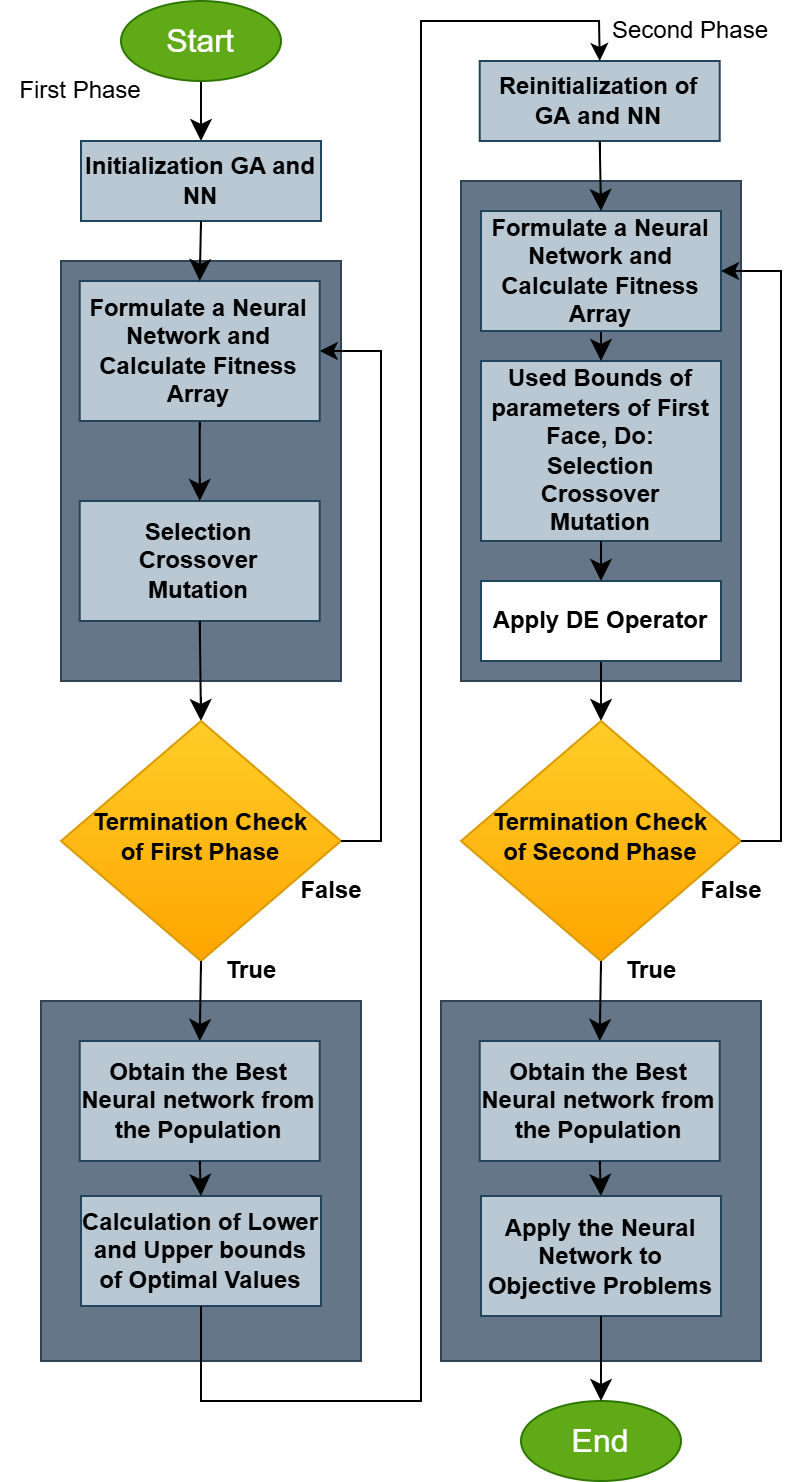
\includegraphics[scale=0.5]{flowChart}
\par\end{centering}
\caption{The flowchart of the proposed method.\protect\label{fig:flow}}

\end{figure}


\section{Experiments \protect\label{sec:Experiments}}

To demonstrate the dynamics and reliability of the proposed methodology,
a series of experiments were carried out on known datasets from the
relevant literature. These datasets were obtained from the following
databases:
\begin{enumerate}
\item The UCI database \url{https://archive.ics.uci.edu/}(accessed on 5
March 2025)\citep{UCL}
\item The Keel website, \url{https://sci2s.ugr.es/keel/datasets.php}(accessed
on 5 March 2025)\citep{Keel}.
\item The Statlib URL \url{ftp://lib.stat.cmu.edu/datasets/index.html }(accessed
on 5 March 2025). 
\end{enumerate}

\subsection{Experimental datasets }

The following series of classification datasets were used in the conducted
experiments:
\begin{enumerate}
\item The Alcohol dataset, which is related to experiments on alcohol consumption
\citep{alcohol}.
\item The Appendicitis dataset, which is a medical dataset \citep{appendicitis}.
\item The Australian dataset, which is used in bank transactions \citep{australian}.
\item The Balance dataset, which contains measurements from various psychological
experiments \citep{balance}.
\item The Circular dataset, which was created artificially. 
\item The Cleveland dataset, which is a medical dataset \citep{cleveland1,cleveland2}.
\item The Dermatology dataset, which is a medical dataset regarding dermatology
problems \citep{dermatology}.
\item The Ecoli dataset, which is used in protein problems \citep{ecoli}.
\item The Fert dataset, related to the detection of relations between sperm
concentration and demographic data.
\item The Haberman dataset, which is related to the detection of breast
cancer.
\item The Hayes roth dataset \citep{hayes-roth}.
\item The Heart dataset, which is related to some heart diseases \citep{heart}. 
\item The HouseVotes dataset, related to data from Congressional voting
in USA \citep{housevotes}.
\item The Ionosphere dataset, that contains measurements from the ionosphere
\citep{ion1,ion2}.
\item The Liverdisorder dataset, which is a medical dataset \citep{liver1,liver2}.
\item The Lymography dataset \citep{lymography}.
\item The Mammographic dataset, which is a medical dataset \citep{mammographic}. 
\item The Parkinsons dataset, that was used in the detection of Parkinson's
disease \citep{parkinsons1,parkinsons2}.
\item The Pima dataset, a medical dataset related to the detection of diabetes's
disease \citep{pima}.
\item The Popfailures dataset, related to climate model simulations \citep{popfailures}.
\item The Regions2 dataset, related to some diseases in liver \citep{regions2}.
\item The Saheart dataset, related to some heart diseases \citep{saheart}.
\item The Segment dataset, related to image processing \citep{segment}.
\item The Sonar dataset, used to discriminate sonar signals \citep{sonar}.
\item The Spiral dataset, which was created artificially. 
\item The StatHeart dataset, a medical dataset regarding heart diseases.
\item The Student dataset, which is related to experiments conducted in
schools \citep{student}.
\item The WDBC dataset, which is related to the detection of cancer \citep{wdbc}.
\item The Wine dataset, used to detection of the quality of wines \citep{wine1,wine2}.
\item The EEG dataset, which contains various EEG measurements \citep{eeg1,eeg2}.
From this dataset the following cases were utilized: Z\_F\_S, ZO\_NF\_S
and ZONF\_S.
\item The ZOO dataset, which is used for animal classification \citep{zoo}.
\end{enumerate}
Also, the following regression datasets were incorporated in the conducted
experiments:
\begin{enumerate}
\item The Abalone dataset, that was used to predict the age of abalones
\citep{abalone}.
\item The Airfoil dataset, derived from NASA \citep{airfoil}.
\item the Baseball dataset, used to predict the salary of baseball players.
\item The BK dataset, related to basketball games \citep{BK}.
\item The BL dataset, related to some electricity experiments.
\item The Concrete dataset, which is related to civil engineering \citep{concrete}.
\item The Dee dataset, which is related to the price of electricity.
\item The Housing dataset, related to the price of houses \citep{housing}.
\item The Friedman dataset, used in various benchmarks \citep{friedman}.
\item The FY dataset, related to fruit flies.
\item The HO dataset, obtained from the STATLIB repository.
\item The Laser dataset, related to laser experiments.
\item The LW dataset, related to the prediction of the weight of babes.
\item The MB dataset, which was obtained from Smoothing Methods in Statistics.
\item The Mortgage dataset, which is an economic dataset.
\item The Plastic dataset, related to the pressure in plastics.
\item The PY dataset \citep{pydataset}.
\item The PL dataset, obtained from the STATLIB repository.
\item The Quake dataset, used to detect the strength of earthquakes. 
\item The SN dataset, which is related to trellising and pruning.
\item The Stock dataset, used to estimate the price of stocks.
\item The Treasury dataset, which is an economic dataset.
\item The VE dataset, obtained from the STATLIB repository.
\end{enumerate}

\subsection{Experimental results}

The code used in the conducted experiments was written in ANSI C++
and all runs were performed 30 times using a different seed for the
random number generator each time. The validation of the experiments
were done using the well - known method of 10 - fold cross validation.
All the experiments were conducted on an AMD RYZEN 5950X machine with
128GB of ram running Debian Linux. For the case of classification
datasets the average classification error is reported in the experimental
tables. This error is calculated through the following equation:
\begin{equation}
E_{C}\left(N(w,x)\right)=100\times\frac{\sum_{i=1}^{K}\left(\mbox{class}\left(N\left(w,x_{i}\right)\right)-y_{i}\right)}{K}
\end{equation}
where the set $T=\left\{ x_{i},y_{i}\right\} ,\ i=1,\ldots,K$ denotes
the test set of the objective problem. For regression datasets the
average regression error as calculated on the test set is reported
and it is denoted as:Also, the regression error is defined as: 
\begin{equation}
E_{R}\left(N(w,x)\right)=\frac{\sum_{i=1}^{K}\left(N\left(w,x_{i}\right)-y_{i}\right)^{2}}{K}
\end{equation}
The values for the parameters of the proposed method are shown in
Table \ref{tab:settings}. In the experimental tables the following
notation is used:
\begin{enumerate}
\item The column DATASET represents the objective problem.
\item The column ADAM denotes the incorporation of the ADAM optimizer \citep{nn_adam}
to train a neural network with $H=10$ processing nodes.
\item The column BFGS represents the application of the BFGS optimizer \citep{powell}
to train a neural network with $H=10$ processing nodes.
\item The column GENETIC denotes the usage of a Genetic Algorithm with the
same set of parameters as shown in Table \ref{tab:settings} to train
an artificial neural network with $H=10$ processing nodes.
\item The column NEAT is used for the application of the NEAT method (NeuroEvolution
of Augmenting Topologies ) \citep{neat}.
\item The row AVERAGE is used for the average classification or regression
error for all datasets.
\end{enumerate}
Also, for the comparisons between methods, the Wilcoxon signed-rank
test was used, a non-parametric test for paired data. Each method
(\textquotedbl PROPOSED\textquotedbl , \textquotedbl BFGS\textquotedbl ,
etc.) was evaluated on the same dataset (dependent measurements),
which is why a paired observations test was selected. The Mann-Whitney
U test or t-test were not applied, as the former is for independent
groups and the latter requires normally distributed data conditions
not met here due to the use of a non-parametric test. 
\begin{table}[H]
\caption{The values of the experimental parameters.\protect\label{tab:settings}}

\centering{}%
\begin{tabular}{|c|c|c|}
\hline 
PARAMETER & MEANING & VALUE\tabularnewline
\hline 
\hline 
$N_{g}$ & Number of generations allowed & 200\tabularnewline
\hline 
$N_{c}$ & Number of chromosomes & 500\tabularnewline
\hline 
$N_{i}$ & Number of generations before the application of the operator & 20\tabularnewline
\hline 
$N_{l}$ & Number of chromosomes where the operator will be applied & 20\tabularnewline
\hline 
$F$ & Differential Weight & 0.8\tabularnewline
\hline 
CR & Crossover probability & 0.9\tabularnewline
\hline 
$p_{s}$ & Selection rate & 0.1\tabularnewline
\hline 
$p_{m}$ & Mutation rate & 0.05\tabularnewline
\hline 
$H$ & Number of processing nodes & 10\tabularnewline
\hline 
$a$ & Margin factor & 1.0\tabularnewline
\hline 
\end{tabular}
\end{table}
The experimental results for the classification datasets are shown
in Table \ref{tab:Experiments-for-classification} and for the regression
datasets in Table \ref{tab:exp2}. 

\begin{table}[H]
\caption{Experimental results for the classification datasets mentioned here
using a series of machine learning methods. The numbers in cells represent
average classification error as reported in the corresponding test
set.\protect\label{tab:Experiments-for-classification}}

\centering{}%
\begin{tabular}{|c|c|c|c|c|c|}
\hline 
DATASET & ADAM & BFGS & NEAT & GENETIC & PROPOSED\tabularnewline
\hline 
\hline 
Alcohol & 57.78\% & 41.50\% & 66.80\% & 39.57\% & 24.79\%\tabularnewline
\hline 
Appendicitis & 16.50\% & 18.00\% & 17.20\% & 18.10\% & 15.97\%\tabularnewline
\hline 
Australian & 35.65\% & 38.13\% & 31.98\% & 32.21\% & 31.76\%\tabularnewline
\hline 
Balance & 7.87\% & 8.64\% & 23.14\% & 8.97\% & 8.39\%\tabularnewline
\hline 
Circular & 19.95\% & 6.08\% & 35.18\% & 5.99\% & 3.69\%\tabularnewline
\hline 
Cleveland & 67.55\% & 77.55\% & 53.44\% & 51.60\% & 48.10\%\tabularnewline
\hline 
Dermatology & 26.14\% & 52.92\% & 32.43\% & 30.58\% & 7.74\%\tabularnewline
\hline 
Ecoli & 64.43\% & 69.52\% & 43.44\% & 54.67\% & 47.62\%\tabularnewline
\hline 
Fert & 23.98\% & 23.20\% & 15.37\% & 28.50\% & 22.00\%\tabularnewline
\hline 
Haberman & 29.00\% & 29.34\% & 24.04\% & 28.66\% & 25.99\%\tabularnewline
\hline 
Hayes Roth & 59.70\% & 37.33\% & 50.15\% & 56.18\% & 37.00\%\tabularnewline
\hline 
Heart & 38.53\% & 39.44\% & 39.27\% & 28.34\% & 24.79\%\tabularnewline
\hline 
HouseVotes & 7.48\% & 7.13\% & 10.89\% & 6.62\% & 5.22\%\tabularnewline
\hline 
Ionosphere & 16.64\% & 15.29\% & 19.67\% & 15.14\% & 9.56\%\tabularnewline
\hline 
Liverdisorder & 41.53\% & 42.59\% & 30.67\% & 31.11\% & 31.08\%\tabularnewline
\hline 
Lymography & 29.26\% & 35.43\% & 33.70\% & 23.26\% & 28.60\%\tabularnewline
\hline 
Mammographic & 46.25\% & 17.24\% & 22.85\% & 19.88\% & 16.98\%\tabularnewline
\hline 
Parkinsons & 24.06\% & 27.58\% & 18.56\% & 18.05\% & 18.02\%\tabularnewline
\hline 
Pima & 34.85\% & 35.59\% & 34.51\% & 32.19\% & 30.44\%\tabularnewline
\hline 
Popfailures & 5.18\% & 5.24\% & 7.05\% & 5.94\% & 4.29\%\tabularnewline
\hline 
Regions2 & 29.85\% & 36.28\% & 33.23\% & 29.39\% & 26.43\%\tabularnewline
\hline 
Saheart & 34.04\% & 37.48\% & 34.51\% & 34.86\% & 32.60\%\tabularnewline
\hline 
Segment & 49.75\% & 68.97\% & 66.72\% & 57.72\% & 30.00\%\tabularnewline
\hline 
Sonar & 30.33\% & 25.85\% & 34.10\% & 22.40\% & 18.78\%\tabularnewline
\hline 
Spiral & 47.67\% & 47.99\% & 48.66\% & 48.66\% & 44.20\%\tabularnewline
\hline 
Statheart & 44.04\% & 39.65\% & 44.36\% & 27.25\% & 22.72\%\tabularnewline
\hline 
Student & 5.13\% & 7.14\% & 10.20\% & 5.61\% & 4.16\%\tabularnewline
\hline 
Wdbc & 35.35\% & 29.91\% & 12.88\% & 8.56\% & 7.73\%\tabularnewline
\hline 
Wine & 29.40\% & 59.71\% & 25.43\% & 19.20\% & 8.55\%\tabularnewline
\hline 
Z\_F\_S & 47.81\% & 39.37\% & 38.41\% & 10.73\% & 6.46\%\tabularnewline
\hline 
ZO\_NF\_S & 47.43\% & 43.04\% & 43.75\% & 21.54\% & 6.01\%\tabularnewline
\hline 
ZONF\_S & 11.99\% & 15.62\% & 5.44\% & 2.60\% & 1.79\%\tabularnewline
\hline 
ZOO & 14.13\% & 10.70\% & 20.27\% & 16.67\% & 9.07\%\tabularnewline
\hline 
\textbf{AVERAGE} & \textbf{32.70\%} & \textbf{33.01\%} & \textbf{31.16\%} & \textbf{25.48\%} & \textbf{20.02\%}\tabularnewline
\hline 
\end{tabular}
\end{table}
\begin{table}[H]
\caption{Experimental results for the regression datasets using a series of
machine learning methods. Numbers in cells stand for the average regression
error as calculated in the corresponding test set.\protect\label{tab:exp2}}

\centering{}%
\begin{tabular}{|c|c|c|c|c|c|}
\hline 
DATASET & ADAM & BFGS & GENETIC & NEAT & PROPOSED\tabularnewline
\hline 
\hline 
ABALONE & 4.30 & 5.69 & 7.17 & 9.88 & 4.33\tabularnewline
\hline 
AIRFOIL & 0.005 & 0.003 & 0.003 & 0.067 & 0.003\tabularnewline
\hline 
BASEBALL & 77.90 & 119.63 & 103.60 & 100.39 & 67.45\tabularnewline
\hline 
BK & 0.03 & 0.28 & 0.027 & 0.15 & 0.02\tabularnewline
\hline 
BL & 0.28 & 2.55 & 5.74 & 0.05 & 0.002\tabularnewline
\hline 
CONCRETE & 0.078 & 0.066 & 0.0099 & 0.081 & 0.003\tabularnewline
\hline 
DEE & 0.63 & 2.36 & 1.013 & 1.512 & 0.20\tabularnewline
\hline 
HOUSING & 80.20 & 97.38 & 43.26 & 56.49 & 26.62\tabularnewline
\hline 
FRIEDMAN & 22.90 & 1.263 & 1.249 & 19.35 & 1.33\tabularnewline
\hline 
FY & 0.038 & 0.22 & 0.65 & 0.08 & 0.039\tabularnewline
\hline 
HO & 0.035 & 0.62 & 2.78 & 0.169 & 0.014\tabularnewline
\hline 
LASER & 0.03 & 0.015 & 0.59 & 0.084 & 0.0027\tabularnewline
\hline 
LW & 0.028 & 2.98 & 1.90 & 0.17 & 0.016\tabularnewline
\hline 
MB & 0.06 & 0.129 & 3.39 & 0.061 & 0.048\tabularnewline
\hline 
MORTGAGE & 9.24 & 8.23 & 2.41 & 14.11 & 0.31\tabularnewline
\hline 
PLASTIC & 11.71 & 20.32 & 2.79 & 20.77 & 2.20\tabularnewline
\hline 
PL & 0.117 & 0.29 & 0.28 & 0.098 & 0.023\tabularnewline
\hline 
PY & 0.09 & 0.578 & 105.41 & 0.075 & 0.016\tabularnewline
\hline 
QUAKE & 0.06 & 0.42 & 0.040 & 0.298 & 0.043\tabularnewline
\hline 
SN & 0.206 & 0.40 & 2.95 & 0.174 & 0.024\tabularnewline
\hline 
STOCK & 180.89 & 302.43 & 3.88 & 215.82 & 3.47\tabularnewline
\hline 
TREASURY & 11.16 & 9.91 & 2.929 & 15.52 & 0.44\tabularnewline
\hline 
VE & 0.359 & 1.92 & 2.43 & 0.045 & 0.023\tabularnewline
\hline 
\textbf{AVERAGE} & \textbf{17.41} & \textbf{25.12} & \textbf{12.80} & \textbf{19.80} & \textbf{4.64}\tabularnewline
\hline 
\end{tabular}
\end{table}
Also, in Figures \ref{fig:statClass} and \ref{fig:statRegression}
the statistical comparison for the experimental results is outlined
graphically.
\begin{figure}[H]
\begin{centering}
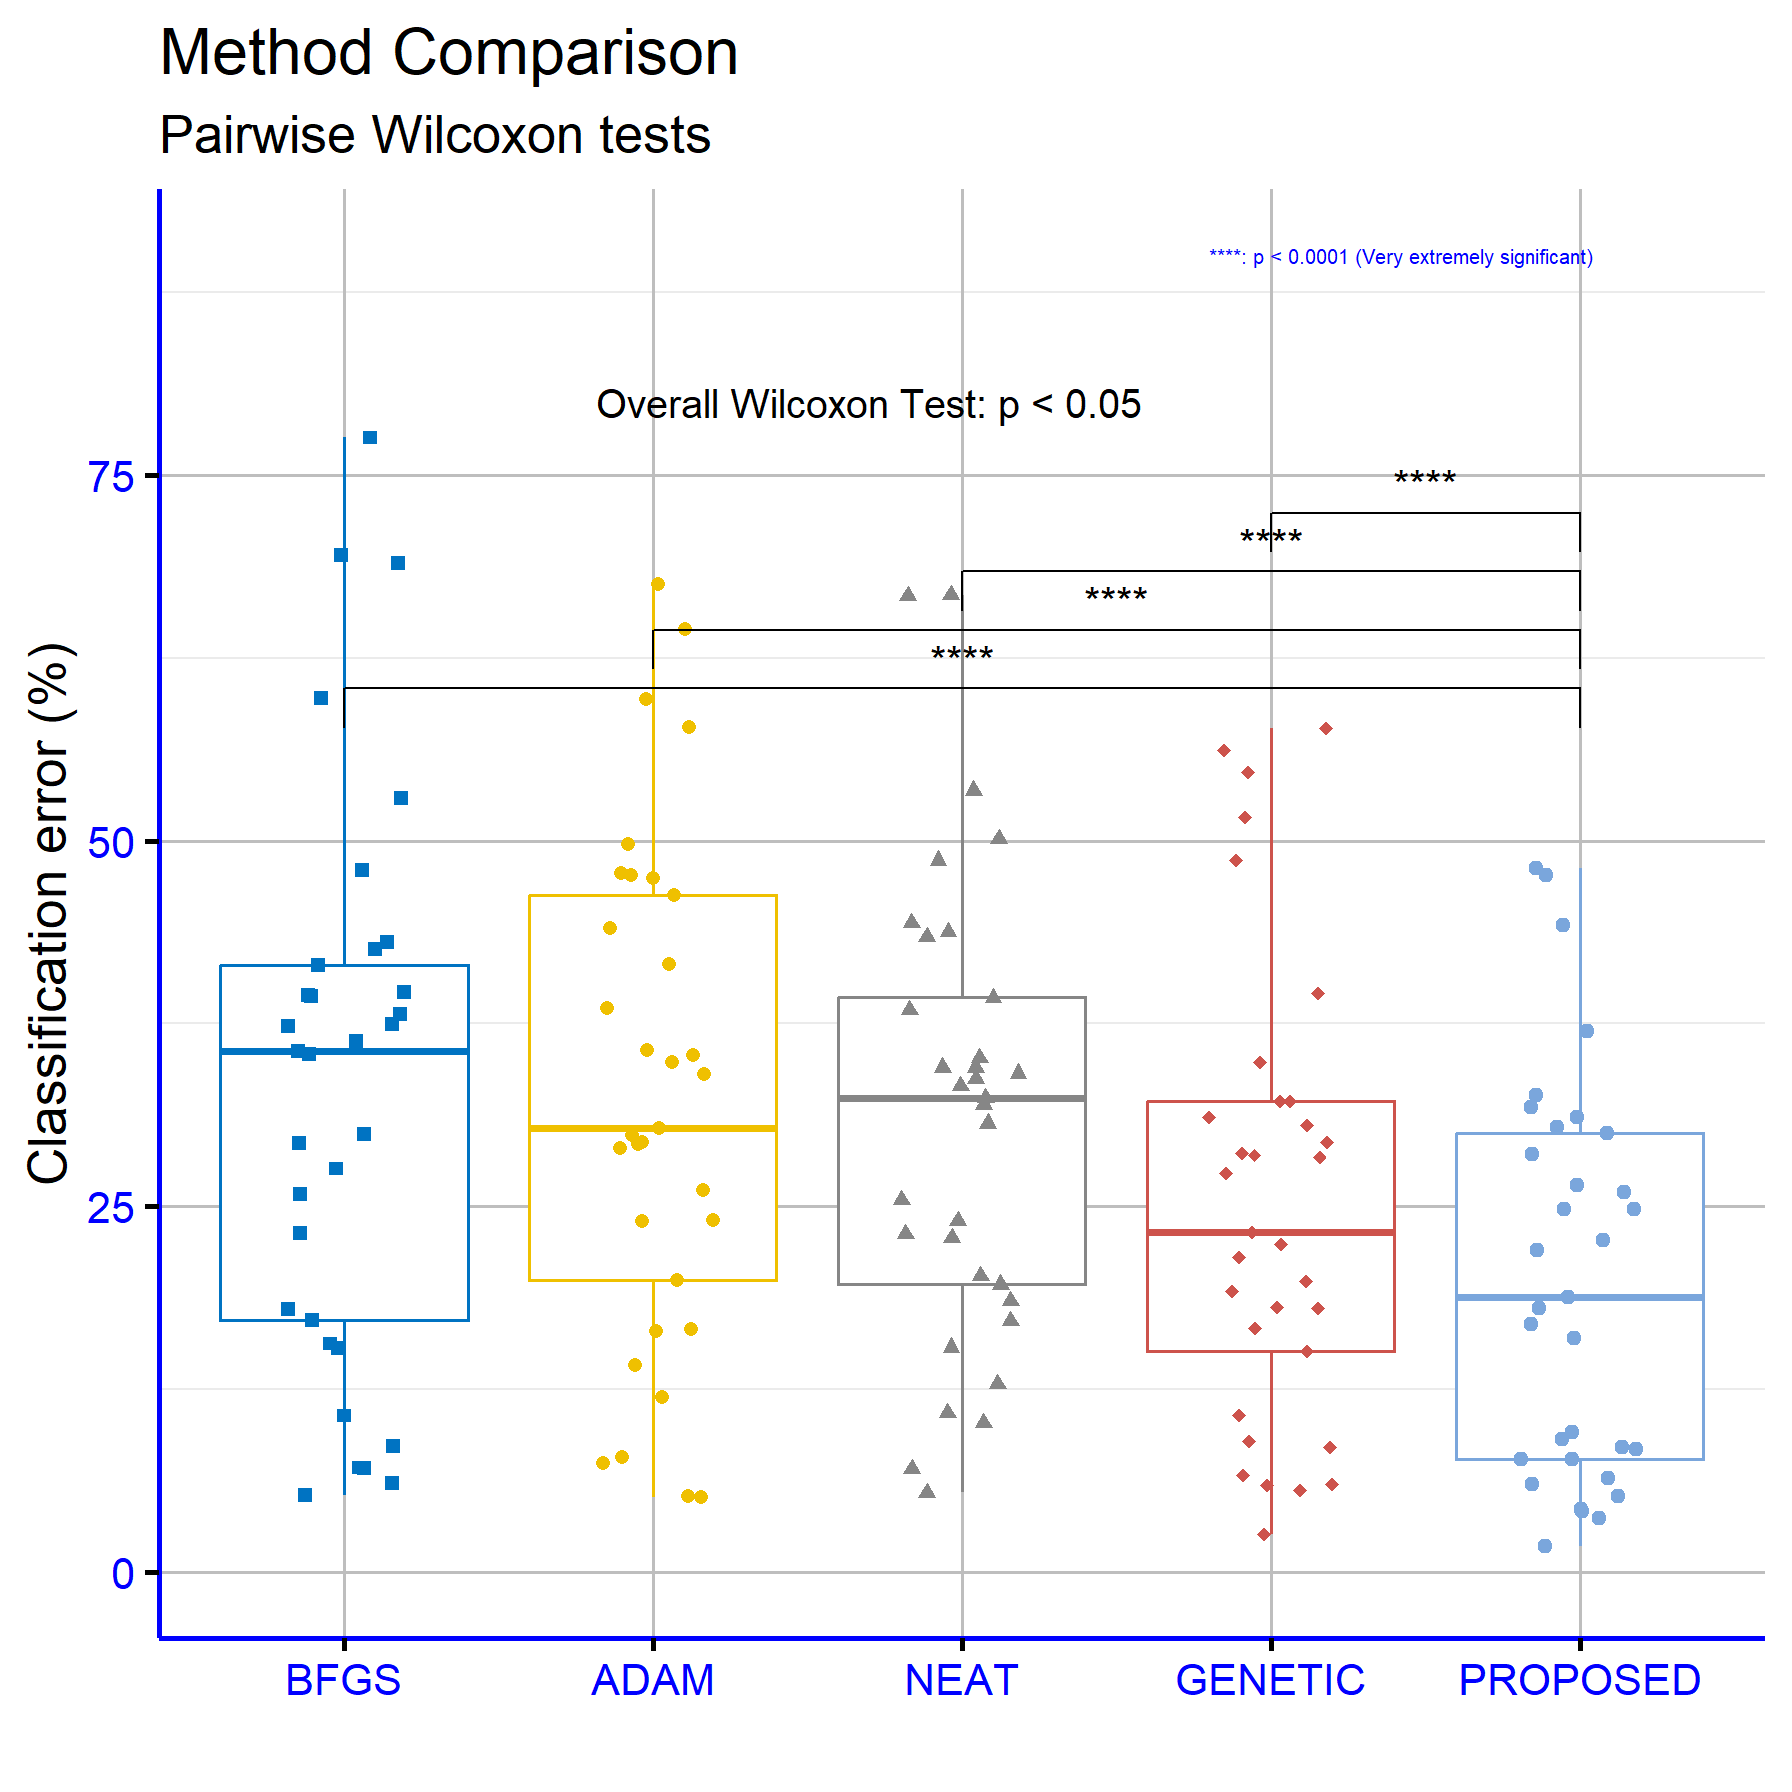
\includegraphics[scale=0.5]{img1}
\par\end{centering}
\caption{Statistical comparison for the obtained experimental results using
a variety of machine learning methods in the classification datasets.\protect\label{fig:statClass}}

\end{figure}
\begin{figure}[H]
\begin{centering}
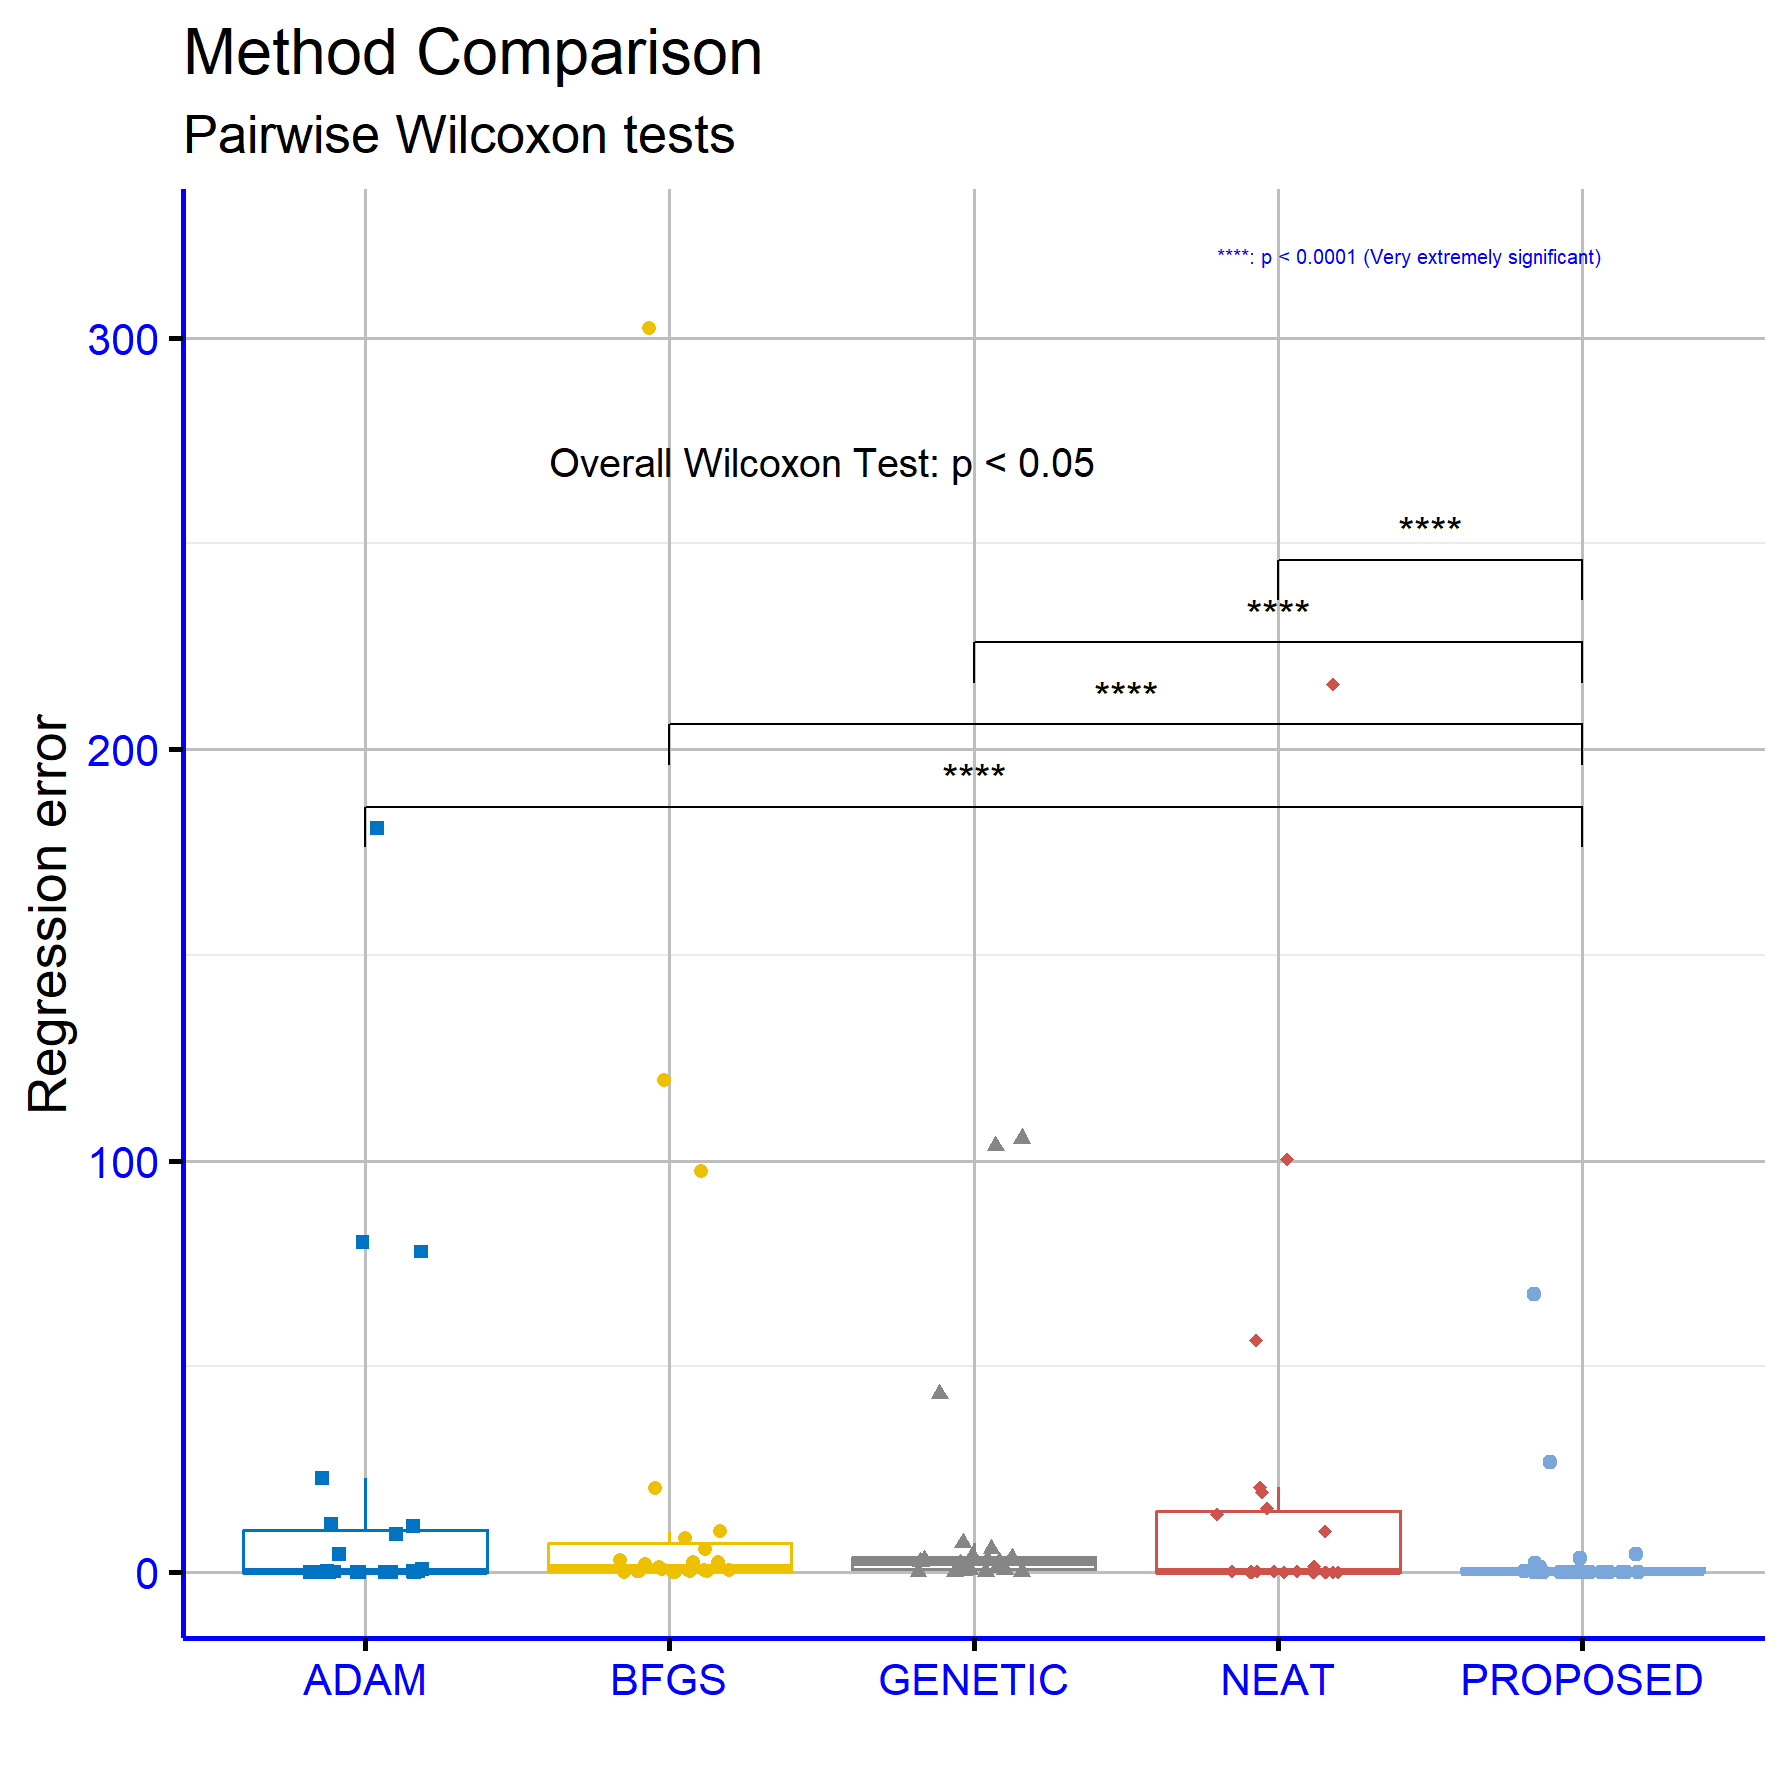
\includegraphics[scale=0.5]{img2}
\par\end{centering}
\caption{Statistical comparison for the experimental results using a series
of machine learning methods on the regression datasets.\protect\label{fig:statRegression}}

\end{figure}
In the scientific analysis of the experimental results, the proposed
model (PROPOSED) demonstrates statistically significant superiority
over other methods (ADAM, BFGS, GENETIC, NEAT, RBF) in both classification
and regression datasets. For classification, the PROPOSED model achieves
a mean error rate of 20.02\%, compared to 25.48\%-33.01\% for the
other methods, with extremely low p-values (e.g., $p=2.3\times10^{-10}$
against BFGS). In regression, the model’s mean absolute error (4.64)
is significantly lower than that of the comparative methods (12.8-25.12),
with strong statistical significance $\left(p<10^{-5}\right)$. However,
in certain datasets (e.g., CLEVELAND, FRIEDMAN), the model’s performance
decreases, indicating dependence on data characteristics.

In the analysis of the experiments (Figure \ref{fig:statClass}) for
classification datasets, the proposed model (PROPOSED) demonstrates
statistically significant superiority over all comparative methods
(BFGS, ADAM, NEAT, GENETIC), with extremely low p-values ($p=2.3\times10^{-10}$
to $p=4.4\times10^{-6}$) . This indicates strong differences at a
confidence level \textgreater 99.9\%, particularly against BFGS and
ADAM $\left(p<10^{-9}\right)$. For regression datasets (Figure \ref{fig:statRegression}),
PROPOSED maintains significant superiority over all methods, though
with slightly higher p-values $\left(p=10^{-5}\ \mbox{to}\ p=2.4\times10^{-7}\right)$.
The largest difference is observed against NEAT $\left(p=2.4\times10^{-7}\right)$,
while the smallest is against GENETIC $\left(p=8.6\times10^{-5}\right)$.

Moreover, in Figure \ref{fig:executionTime}the a comparison of execution
times is graphically outlined between the simple Genetic algorithm
and the proposed method for various values of the critical parameter
$N_{I}$. The dataset used in this experiment is the WINE classification
dataset. As expected, increasing the value for this parameter also
leads to a reduction in the required execution time for the proposed
method, since the new genetic operator is applied more and more sparsely
to the population chromosomes.

\begin{figure}[H]
\begin{centering}
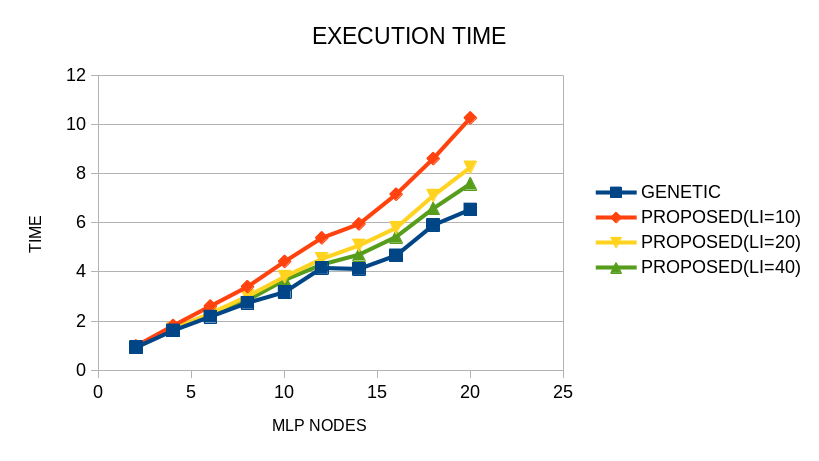
\includegraphics[scale=0.5]{execution_time}
\par\end{centering}
\caption{Comparison of execution times for the WINE dataset between the simple
Genetic algorithm and the proposed method for various values of the
parameter $N_{I}$.\protect\label{fig:executionTime}}

\end{figure}


\subsection{Experiments with the differential weight }

An additional experiment was performed to demonstrate the reliability
of the proposed methodology. In this experiment, three different differential
weight $F$ calculation techniques were used for the proposed operator.
The range of this parameter was defined as $[0,2]$ in the work of
Storn and Price \citep{de_original}. These techniques are the following:
\begin{enumerate}
\item Fixed, which is the default technique in the proposed method. In this
technique the value $F=0.8$ is used for the differential weight.
\item Adaptive, where the adaptive calculation of parameter $F$ is uses
as proposed in \citep{de_adaptive}.
\item Random, where the stochastic calculation of parameter $F$ as proposed
in \citep{de_char} is used.
\end{enumerate}
In table \ref{tab:ExperimentsClassificationF} the results from the
application of the proposed method using the previously mentioned
techniques for the differential weight are depicted for the classification
datasets. Similarly, the same method is applied on the regression
datasets and the results are presented in Table \ref{tab:expRegressionF}.

\begin{table}[H]
\caption{Experiments for classification datasets using a series of differential
weight mechanisms.\protect\label{tab:ExperimentsClassificationF}}

\centering{}%
\begin{tabular}{|c|c|c|c|}
\hline 
DATASET & FIXED & ADAPTIVE & RANDOM\tabularnewline
\hline 
\hline 
Alcohol & 24.79\% & 25.65\% & 23.02\%\tabularnewline
\hline 
Appendicitis & 15.97\% & 15.83\% & 15.80\%\tabularnewline
\hline 
Australian & 31.76\% & 31.61\% & 31.60\%\tabularnewline
\hline 
Balance & 8.39\% & 8.45\% & 8.65\%\tabularnewline
\hline 
Circular & 3.69\% & 3.67\% & 3.78\%\tabularnewline
\hline 
Cleveland & 48.10\% & 48.39\% & 48.35\%\tabularnewline
\hline 
Dermatology & 7.74\% & 7.27\% & 7.37\%\tabularnewline
\hline 
Ecoli & 47.62\% & 48.34\% & 47.96\%\tabularnewline
\hline 
Fert & 22.00\% & 22.17\% & 22.10\%\tabularnewline
\hline 
Haberman & 25.99\% & 26.20\% & 26.12\%\tabularnewline
\hline 
Hayes Roth & 37.00\% & 38.38\% & 37.65\%\tabularnewline
\hline 
Heart & 24.79\% & 24.15\% & 25.51\%\tabularnewline
\hline 
HouseVotes & 5.22\% & 5.21\% & 4.78\%\tabularnewline
\hline 
Ionosphere & 9.56\% & 9.28\% & 9.30\%\tabularnewline
\hline 
Liverdisorder & 31.08\% & 31.46\% & 31.11\%\tabularnewline
\hline 
Lymography & 28.60\% & 28.95\% & 27.88\%\tabularnewline
\hline 
Mammographic & 16.98\% & 17.02\% & 17.18\%\tabularnewline
\hline 
Parkinsons & 18.02\% & 17.86\% & 17.90\%\tabularnewline
\hline 
Pima & 30.44\% & 31.12\% & 30.48\%\tabularnewline
\hline 
Popfailures & 4.29\% & 4.25\% & 4.28\%\tabularnewline
\hline 
Regions2 & 26.43\% & 25.94\% & 26.35\%\tabularnewline
\hline 
Saheart & 32.60\% & 33.11\% & 32.92\%\tabularnewline
\hline 
Segment & 30.00\% & 28.83\% & 30.85\%\tabularnewline
\hline 
Sonar & 18.78\% & 18.08\% & 18.70\%\tabularnewline
\hline 
Spiral & 44.20\% & 44.21\% & 44.12\%\tabularnewline
\hline 
Statheart & 22.72\% & 22.72\% & 23.41\%\tabularnewline
\hline 
Student & 4.16\% & 3.95\% & 4.35\%\tabularnewline
\hline 
Wdbc & 7.73\% & 7.48\% & 7.40\%\tabularnewline
\hline 
Wine & 8.55\% & 6.29\% & 6.74\%\tabularnewline
\hline 
Z\_F\_S & 6.46\% & 6.92\% & 6.65\%\tabularnewline
\hline 
ZO\_NF\_S & 6.01\% & 6.10\% & 5.89\%\tabularnewline
\hline 
ZONF\_S & 1.79\% & 1.71\% & 1.76\%\tabularnewline
\hline 
ZOO & 9.07\% & 6.57\% & 8.90\%\tabularnewline
\hline 
\textbf{AVERAGE} & \textbf{20.02\%} & \textbf{19.91\%} & \textbf{19.97\%}\tabularnewline
\hline 
\end{tabular}
\end{table}
\begin{table}[H]
\caption{Experiments for regression datasets using a variety of weight mechanism
methods.\protect\label{tab:expRegressionF}}

\centering{}%
\begin{tabular}{|c|c|c|c|}
\hline 
DATASET & FIXED & ADAPTIVE & RANDOM\tabularnewline
\hline 
\hline 
ABALONE & 4.33 & 4.24 & 4.34\tabularnewline
\hline 
AIRFOIL & 0.003 & 0.003 & 0.003\tabularnewline
\hline 
BASEBALL & 67.45 & 67.23 & 66.76\tabularnewline
\hline 
BK & 0.02 & 0.02 & 0.02\tabularnewline
\hline 
BL & 0.002 & 0.002 & 0.002\tabularnewline
\hline 
CONCRETE & 0.003 & 0.003 & 0.003\tabularnewline
\hline 
DEE & 0.20 & 0.20 & 0.20\tabularnewline
\hline 
HOUSING & 26.62 & 26.07 & 26.11\tabularnewline
\hline 
FRIEDMAN & 1.33 & 1.21 & 1.34\tabularnewline
\hline 
FY & 0.039 & 0.039 & 0.039\tabularnewline
\hline 
HO & 0.014 & 0.014 & 0.014\tabularnewline
\hline 
LASER & 0.0027 & 0.0027 & 0.0028\tabularnewline
\hline 
LW & 0.016 & 0.011 & 0.011\tabularnewline
\hline 
MB & 0.048 & 0.048 & 0.048\tabularnewline
\hline 
MORTGAGE & 0.31 & 0.35 & 0.34\tabularnewline
\hline 
PLASTIC & 2.20 & 2.13 & 2.20\tabularnewline
\hline 
PL & 0.023 & 0.022 & 0.022\tabularnewline
\hline 
PY & 0.016 & 0.017 & 0.017\tabularnewline
\hline 
QUAKE & 0.043 & 0.082 & 0.04\tabularnewline
\hline 
SN & 0.024 & 0.024 & 0.024\tabularnewline
\hline 
STOCK & 3.47 & 3.33 & 3.45\tabularnewline
\hline 
TREASURY & 0.44 & 0.42 & 0.45\tabularnewline
\hline 
VE & 0.023 & 0.023 & 0.023\tabularnewline
\hline 
\textbf{AVERAGE} & \textbf{4.64} & \textbf{4.59} & \textbf{4.59}\tabularnewline
\hline 
\end{tabular}
\end{table}
Furthermore, the statistical comparison for these experimental tables
is outlined in Figures \ref{fig:statClassF} and \ref{fig:statRegressionF}
respectively.

\begin{figure}[H]
\begin{centering}
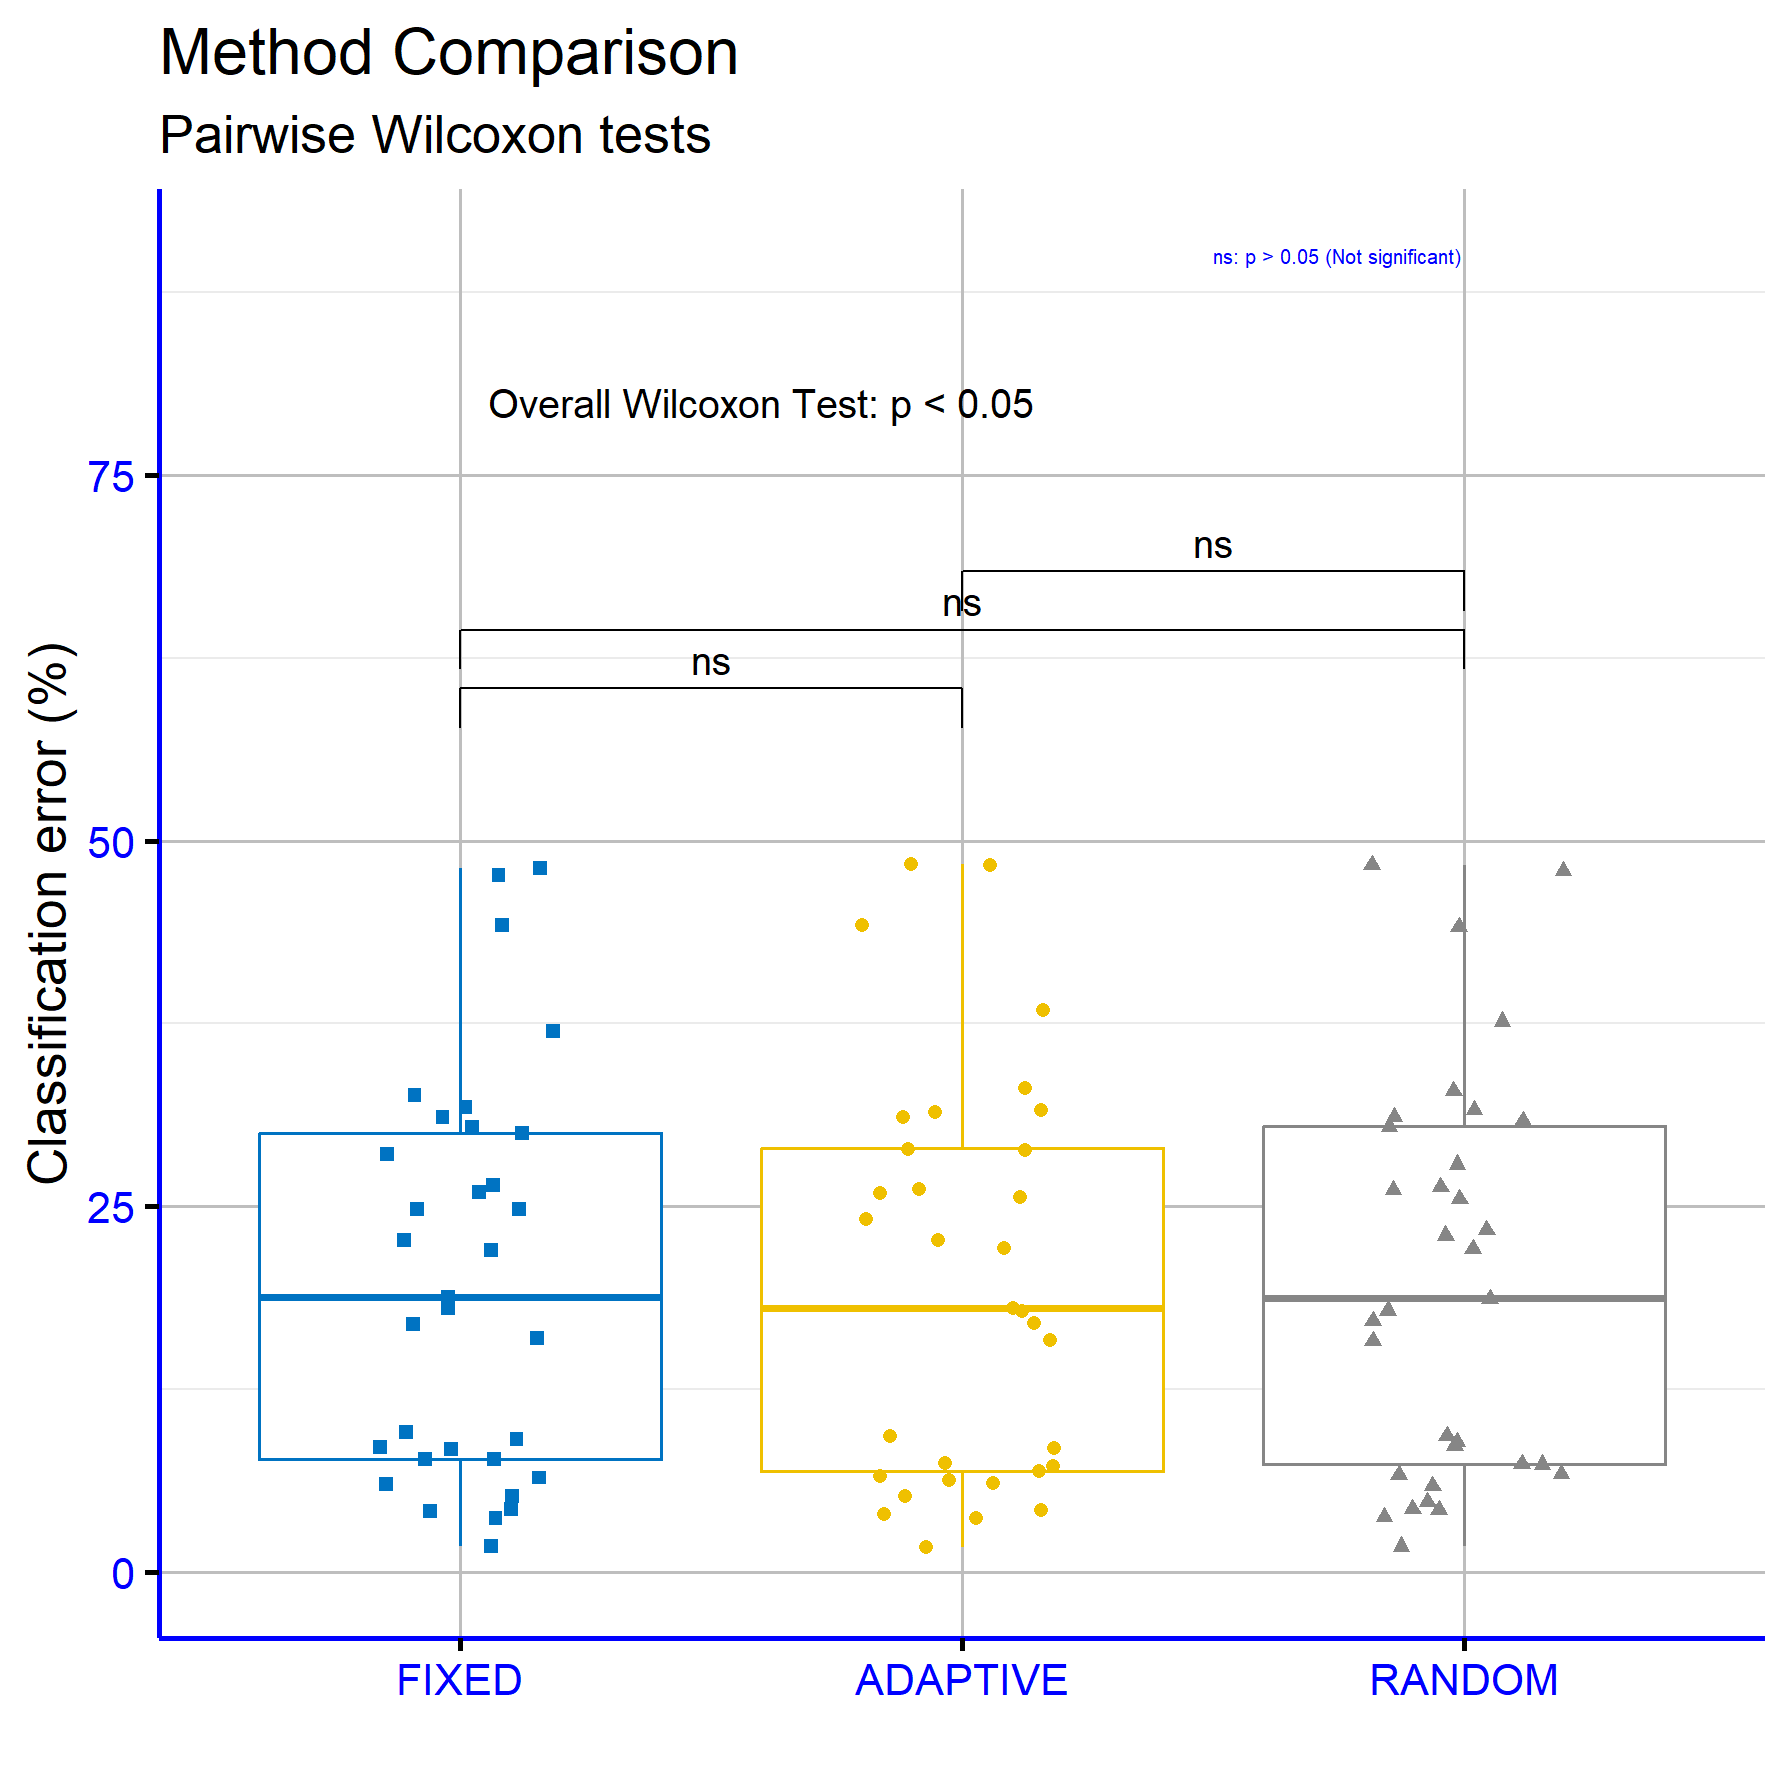
\includegraphics[scale=0.5]{img3}
\par\end{centering}
\caption{Statistical comparison for the experimental results on the classification
datasets, using the proposed method and a series of differential weight
techniques.\protect\label{fig:statClassF}}

\end{figure}
\begin{figure}[H]
\begin{centering}
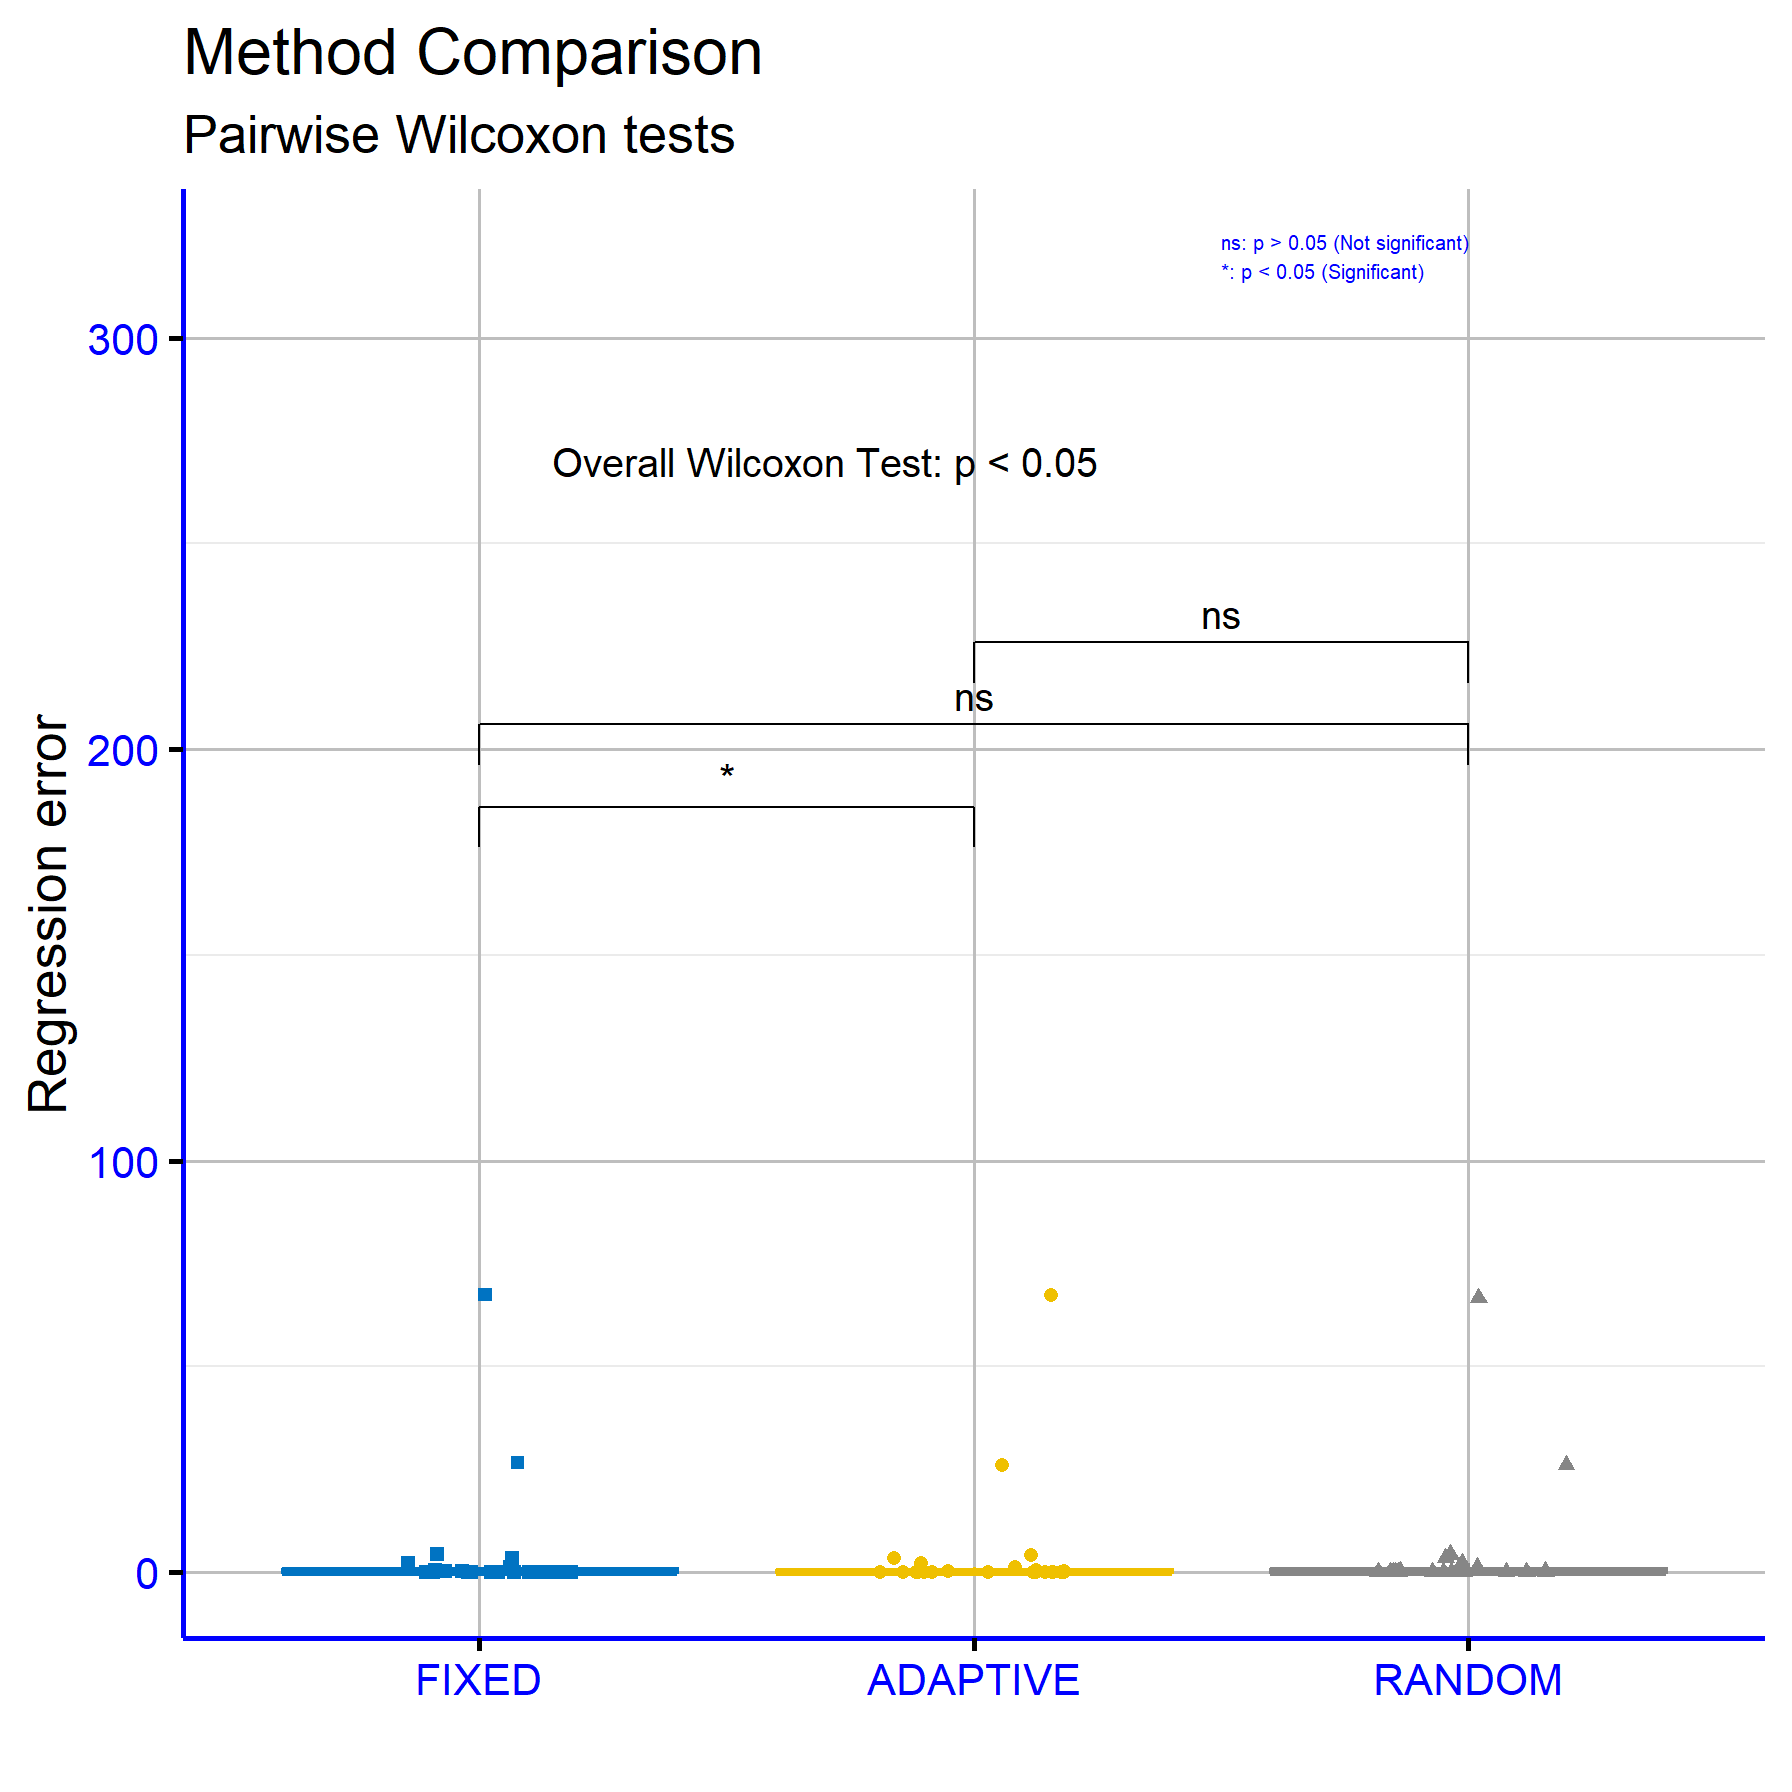
\includegraphics[scale=0.5]{img4}
\par\end{centering}
\caption{Statistical comparison for the experiments on the regression datasets
using the proposed method and a series of differential weight calculation
techniques.\protect\label{fig:statRegressionF}}

\end{figure}
When comparing differential weight calculation methods (FIXED, ADAPTIVE,
RANDOM), the ADAPTIVE method shows slightly better average performance
(19.91\% in classification, 4.59 in regression) compared to FIXED
(20.02\%, 4.64) and RANDOM (19.97\%, 4.59). However, the differences
are minimal and often statistically insignificant (e.g., $p=0.83$for
FIXED vs ADAPTIVE in classification). In some datasets, such as Lymography
and HouseVotes, the RANDOM method outperforms others, highlighting
the need to tailor the method to the specific problem. In regression,
the only significant difference occurs between FIXED and ADAPTIVE
($p=0.041$).

For this experiment as shown in Figure \ref{fig:statClassF}, the
differences between FIXED and ADAPTIVE ($p=0.83$) and ADAPTIVE vs
RANDOM ($p=0.94$) are not statistically significant, suggesting equivalent
performance. However, the comparison FIXED vs RANDOM ($p=2.3\times10^{-10}$)
reveals a highly significant difference, likely due to the random
nature of RANDOM. For regression datasets (Figure \ref{fig:statRegressionF}),
the only significant difference occurs between FIXED and ADAPTIVE
($p=0.041$), while the remaining comparisons (FIXED vs RANDOM: $p=0.75$,
ADAPTIVE vs RANDOM: $p=0.31$) lack statistical significance.

\subsection{Experiments with the margin factor $a$}

An additional experiment was executed to outline the performance and
the stability of the proposed method. In this experiment that margin
factor denoted as $a$ in the proposed method was varied from $a=1.0$
(which is the default value) to $a=4.0$. The experimental results
for the classification datasets are shown in Table \ref{tab:ExperimentsClassificationA}
and for regression datasets in Table \ref{tab:expRegressionA}.

\begin{table}[H]
\caption{Experiments for classification datasets using a series of values for
the margin factor $a$.\protect\label{tab:ExperimentsClassificationA}}

\centering{}%
\begin{tabular}{|c|c|c|c|c|c|c|c|}
\hline 
DATASET & $a=1.0$ & $a=1.5$ & $a=2.0$ & $a=2.5$ & $a=3.0$ & $a=3.5$ & $a=4.0$\tabularnewline
\hline 
\hline 
Alcohol & 24.79\% & 22.88\% & 25.55\% & 30.21\% & 30.77\% & 32.05\% & 28.42\%\tabularnewline
\hline 
Appendicitis & 15.97\% & 16.33\% & 18.07\% & 18.70\% & 17.30\% & 18.60\% & 19.51\%\tabularnewline
\hline 
Australian & 31.76\% & 32.79\% & 33.23\% & 32.65\% & 32.87\% & 32.76\% & 33.68\%\tabularnewline
\hline 
Balance & 8.39\% & 8.50\% & 8.39\% & 8.84\% & 8.85\% & 8.87\% & 8.78\%\tabularnewline
\hline 
Circular & 3.69\% & 4.19\% & 4.22\% & 4.30\% & 4.33\% & 4.46\% & 4.70\%\tabularnewline
\hline 
Cleveland & 48.10\% & 47.17\% & 46.68\% & 47.58\% & 50.84\% & 50.62\% & 47.74\%\tabularnewline
\hline 
Dermatology & 7.74\% & 7.47\% & 7.60\% & 7.57\% & 7.71\% & 8.86\% & 7.83\%\tabularnewline
\hline 
Ecoli & 47.62\% & 48.69\% & 48.29\% & 49.50\% & 51.39\% & 51.99\% & 49.39\%\tabularnewline
\hline 
Fert & 22.00\% & 23.47\% & 23.50\% & 25.03\% & 24.80\% & 24.17\% & 24.27\%\tabularnewline
\hline 
Haberman & 25.99\% & 26.26\% & 26.74\% & 27.23\% & 27.49\% & 27.67\% & 27.14\%\tabularnewline
\hline 
Hayes Roth & 37.00\% & 39.15\% & 39.69\% & 35.49\% & 38.10\% & 39.15\% & 40.05\%\tabularnewline
\hline 
Heart & 24.79\% & 24.64\% & 24.85\% & 25.50\% & 26.85\% & 26.46\% & 24.89\%\tabularnewline
\hline 
HouseVotes & 5.22\% & 4.91\% & 5.05\% & 4.90\% & 4.57\% & 4.71\% & 5.02\%\tabularnewline
\hline 
Ionosphere & 9.56\% & 9.65\% & 9.92\% & 9.72\% & 9.75\% & 9.57\% & 10.23\%\tabularnewline
\hline 
Liverdisorder & 31.08\% & 31.94\% & 31.42\% & 30.89\% & 31.54\% & 30.92\% & 32.13\%\tabularnewline
\hline 
Lymography & 28.60\% & 28.24\% & 28.79\% & 30.21\% & 29.64\% & 30.71\% & 26.69\%\tabularnewline
\hline 
Mammographic & 16.98\% & 16.34\% & 16.35\% & 15.86\% & 15.88\% & 16.35\% & 16.69\%\tabularnewline
\hline 
Parkinsons & 18.02\% & 18.88\% & 18.56\% & 17.98\% & 17.74\% & 17.95\% & 19.40\%\tabularnewline
\hline 
Pima & 30.44\% & 30.89\% & 31.11\% & 32.81\% & 32.88\% & 32.83\% & 31.03\%\tabularnewline
\hline 
Popfailures & 4.29\% & 5.07\% & 5.53\% & 5.51\% & 5.54\% & 5.97\% & 5.97\%\tabularnewline
\hline 
Regions2 & 26.43\% & 26.53\% & 26.30\% & 26.52\% & 26.28\% & 26.26\% & 25.35\%\tabularnewline
\hline 
Saheart & 32.60\% & 31.43\% & 32.98\% & 33.52\% & 33.49\% & 33.46\% & 32.93\%\tabularnewline
\hline 
Segment & 30.00\% & 27.98\% & 30.86\% & 31.39\% & 33.76\% & 34.51\% & 35.41\%\tabularnewline
\hline 
Sonar & 18.78\% & 21.08\% & 22.23\% & 21.47\% & 21.75\% & 21.57\% & 21.68\%\tabularnewline
\hline 
Spiral & 44.20\% & 44.65\% & 44.52\% & 43.81\% & 43.58\% & 43.39\% & 44.13\%\tabularnewline
\hline 
Statheart & 22.72\% & 23.40\% & 23.85\% & 24.22\% & 25.56\% & 26.10\% & 24.22\%\tabularnewline
\hline 
Student & 4.16\% & 4.75\% & 5.24\% & 5.38\% & 5.43\% & 5.55\% & 5.37\%\tabularnewline
\hline 
Wdbc & 7.73\% & 6.95\% & 6.64\% & 7.14\% & 7.29\% & 7.17\% & 7.31\%\tabularnewline
\hline 
Wine & 8.55\% & 6.59\% & 9.35\% & 9.47\% & 8.12\% & 9.65\% & 11.02\%\tabularnewline
\hline 
Z\_F\_S & 6.46\% & 6.66\% & 6.90\% & 6.92\% & 6.53\% & 6.87\% & 6.61\%\tabularnewline
\hline 
ZO\_NF\_S & 6.01\% & 6.03\% & 6.08\% & 6.95\% & 7.17\% & 7.28\% & 6.25\%\tabularnewline
\hline 
ZONF\_S & 1.79\% & 1.75\% & 1.80\% & 2.15\% & 2.14\% & 2.13\% & 1.79\%\tabularnewline
\hline 
ZOO & 9.07\% & 8.63\% & 7.00\% & 7.87\% & 6.77\% & 6.97\% & 7.53\%\tabularnewline
\hline 
\textbf{AVERAGE} & \textbf{20.02\%} & \textbf{20.12\%} & \textbf{20.52\%} & \textbf{20.83\%} & \textbf{21.11\%} & \textbf{21.38\%} & \textbf{21.00\%}\tabularnewline
\hline 
\end{tabular}
\end{table}
\begin{table}[H]
\caption{Experiments for regression datasets using a variety of values for
the margin factor $a$.\protect\label{tab:expRegressionA}}

\centering{}%
\begin{tabular}{|c|c|c|c|c|c|c|c|}
\hline 
DATASET & $a=1.0$ & $a=1.5$ & $a=2.0$ & $a=2.5$ & $a=3.0$ & $a=3.5$ & $a=4.0$\tabularnewline
\hline 
\hline 
ABALONE & 4.33 & 4.39 & 4.46 & 4.64 & 4.84 & 4.93 & 5.06\tabularnewline
\hline 
AIRFOIL & 0.003 & 0.003 & 0.002 & 0.002 & 0.003 & 0.003 & 0.002\tabularnewline
\hline 
BASEBALL & 67.45 & 74.66 & 79.78 & 79.39 & 81.55 & 84.65 & 86.54\tabularnewline
\hline 
BK & 0.02 & 0.019 & 0.019 & 0.018 & 0.017 & 0.018 & 0.02\tabularnewline
\hline 
BL & 0.002 & 0.001 & 0.001 & 0.0007 & 0.0009 & 0.0008 & 0.003\tabularnewline
\hline 
CONCRETE & 0.003 & 0.003 & 0.003 & 0.004 & 0.003 & 0.004 & 0.003\tabularnewline
\hline 
DEE & 0.20 & 0.20 & 0.20 & 0.21 & 0.20 & 0.21 & 0.20\tabularnewline
\hline 
HOUSING & 26.62 & 26.24 & 28.13 & 27.91 & 27.36 & 29.53 & 29.25\tabularnewline
\hline 
FRIEDMAN & 1.33 & 1.19 & 1.20 & 1.21 & 1.22 & 1.21 & 1.20\tabularnewline
\hline 
FY & 0.039 & 0.04 & 0.042 & 0.041 & 0.042 & 0.042 & 0.045\tabularnewline
\hline 
HO & 0.014 & 0.014 & 0.013 & 0.013 & 0.013 & 0.014 & 0.014\tabularnewline
\hline 
LASER & 0.0027 & 0.0025 & 0.0025 & 0.0028 & 0.0026 & 0.0025 & 0.0024\tabularnewline
\hline 
LW & 0.016 & 0.011 & 0.011 & 0.013 & 0.013 & 0.014 & 0.013\tabularnewline
\hline 
MB & 0.048 & 0.049 & 0.051 & 0.051 & 0.052 & 0.054 & 0.09\tabularnewline
\hline 
MORTGAGE & 0.31 & 0.21 & 0.37 & 0.48 & 0.63 & 0.68 & 0.62\tabularnewline
\hline 
PLASTIC & 2.20 & 2.05 & 2.18 & 2.23 & 2.25 & 2.23 & 2.21\tabularnewline
\hline 
PL & 0.023 & 0.023 & 0.021 & 0.022 & 0.022 & 0.022 & 0.022\tabularnewline
\hline 
PY & 0.016 & 0.022 & 0.023 & 0.026 & 0.028 & 0.027 & 0.028\tabularnewline
\hline 
QUAKE & 0.043 & 0.038 & 0.04 & 0.039 & 0.037 & 0.037 & 0.039\tabularnewline
\hline 
SN & 0.024 & 0.024 & 0.025 & 0.024 & 0.026 & 0.024 & 0.026\tabularnewline
\hline 
STOCK & 3.47 & 3.59 & 3.68 & 3.70 & 3.37 & 3.24 & 3.35\tabularnewline
\hline 
TREASURY & 0.44 & 0.42 & 0.40 & 0.65 & 0.82 & 0.95 & 1.01\tabularnewline
\hline 
VE & 0.023 & 0.024 & 0.024 & 0.025 & 0.026 & 0.027 & 0.029\tabularnewline
\hline 
\textbf{AVERAGE} & \textbf{4.64} & \textbf{4.92} & \textbf{5.25} & \textbf{5.25} & \textbf{5.33} & \textbf{5.56} & \textbf{5.64}\tabularnewline
\hline 
\end{tabular}
\end{table}
Also, the statistical comparisons for these experiments are shown
graphically in Figures \ref{fig:statClassA} and \ref{fig:statRegressionA}
respectively. 

\begin{figure}[H]
\begin{centering}
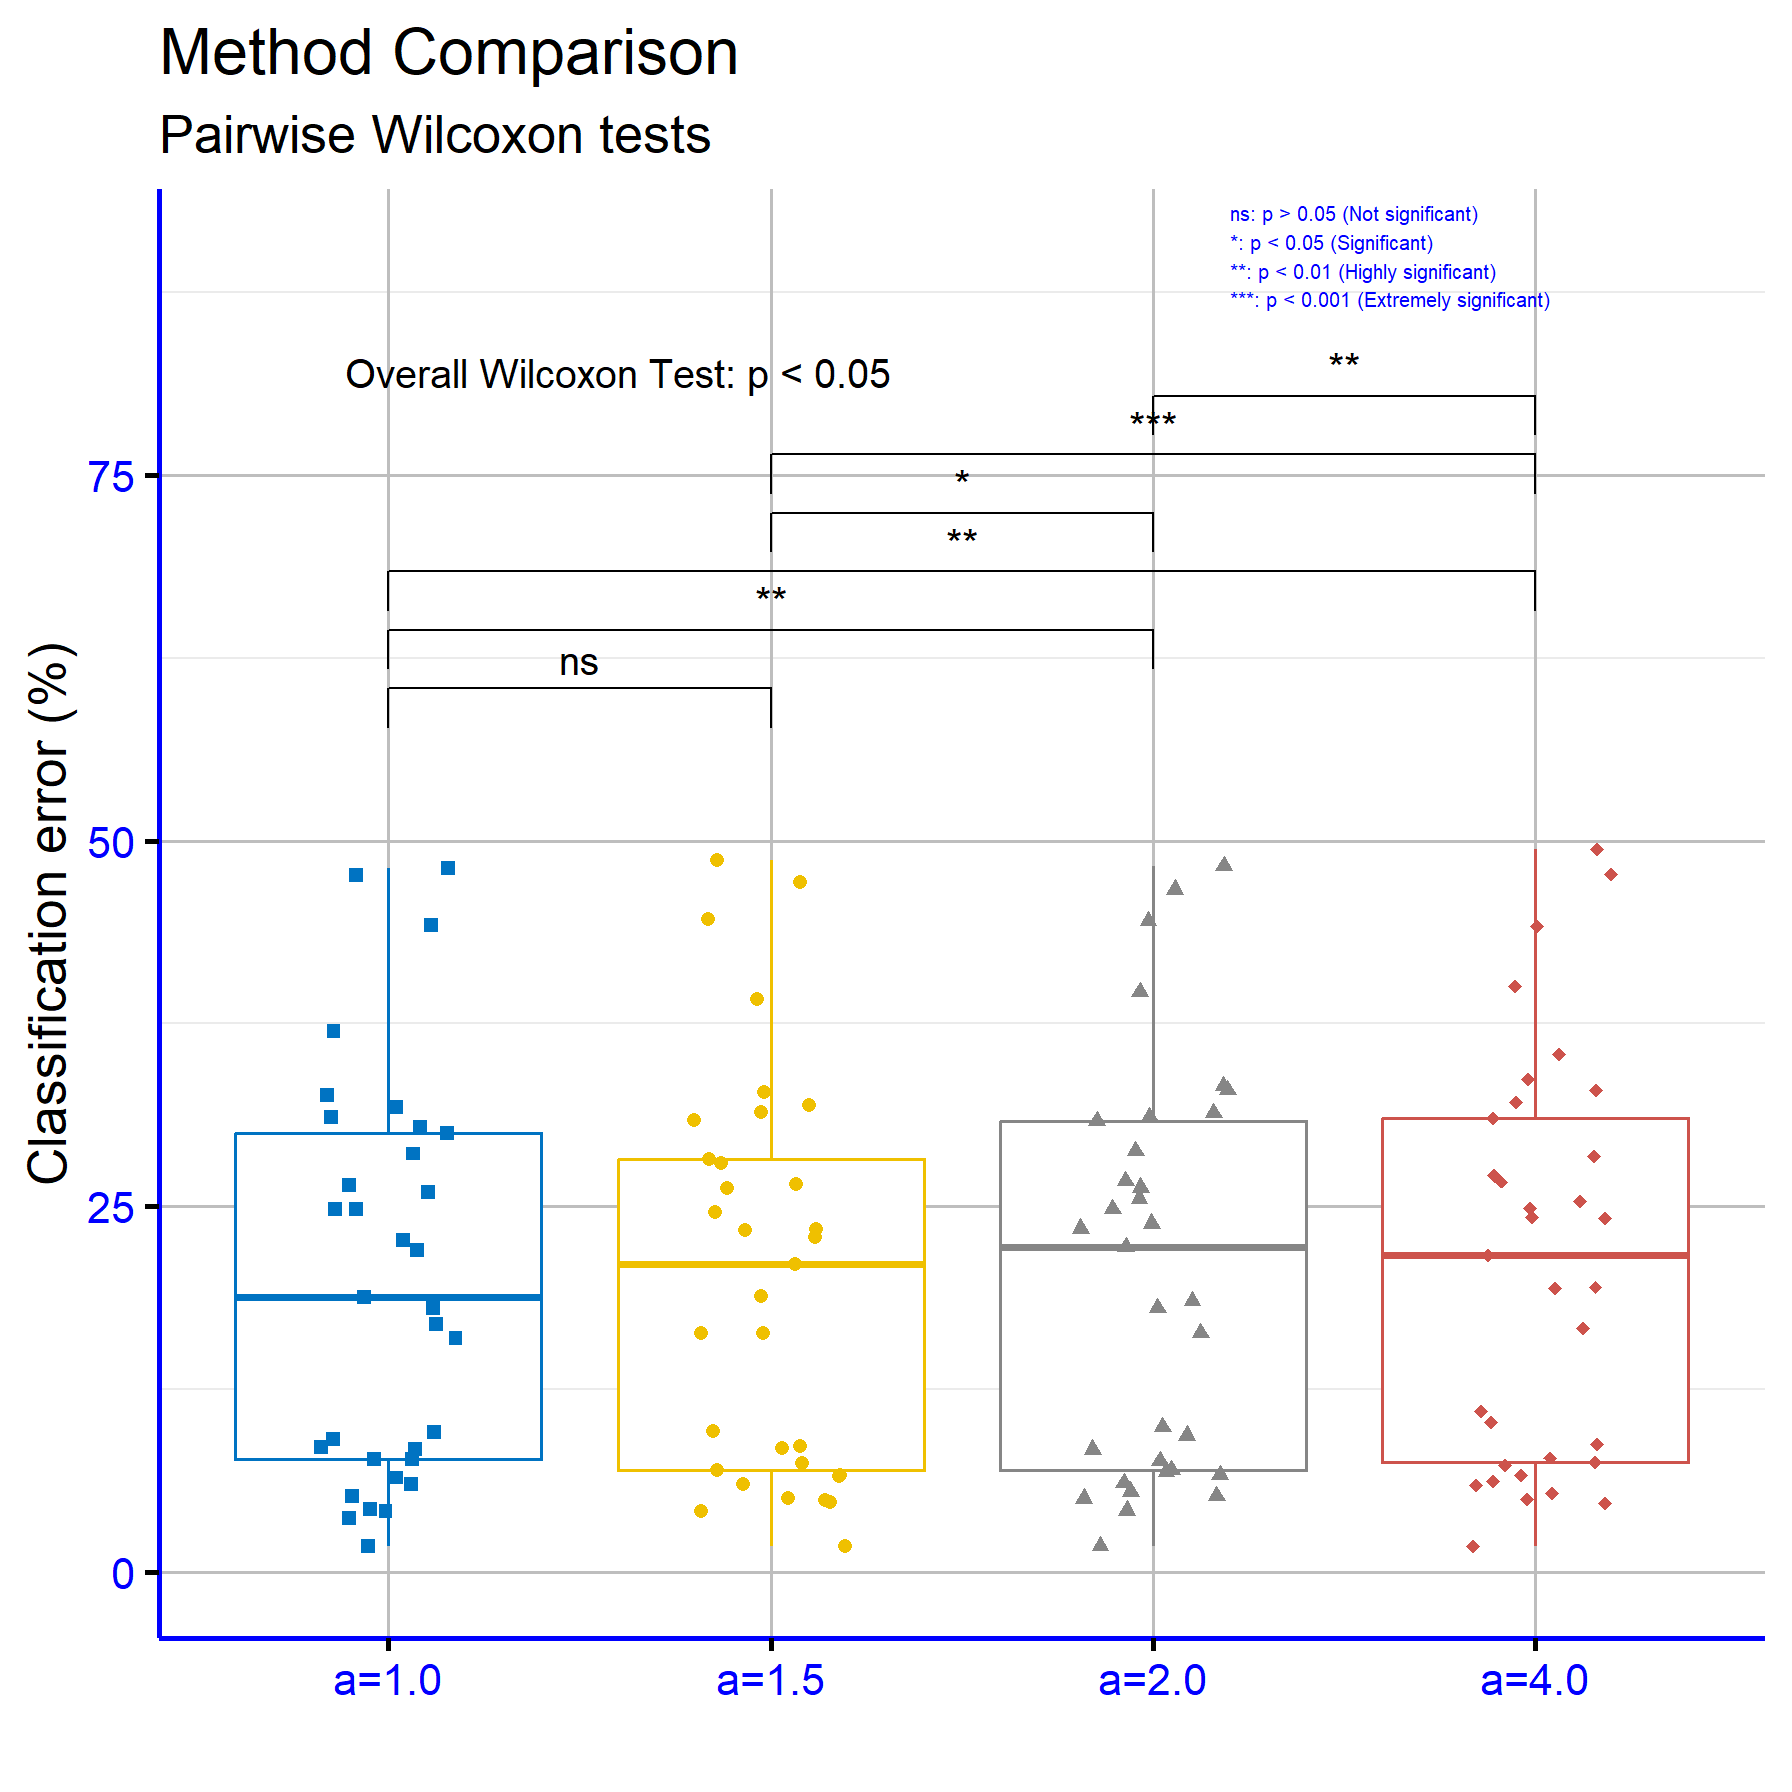
\includegraphics[scale=0.5]{img5}
\par\end{centering}
\caption{Statistical comparison for the experimental results on the classification
datasets, using the proposed method and different values for the margin
factor $a$.\protect\label{fig:statClassA}}

\end{figure}
\begin{figure}[H]
\begin{centering}
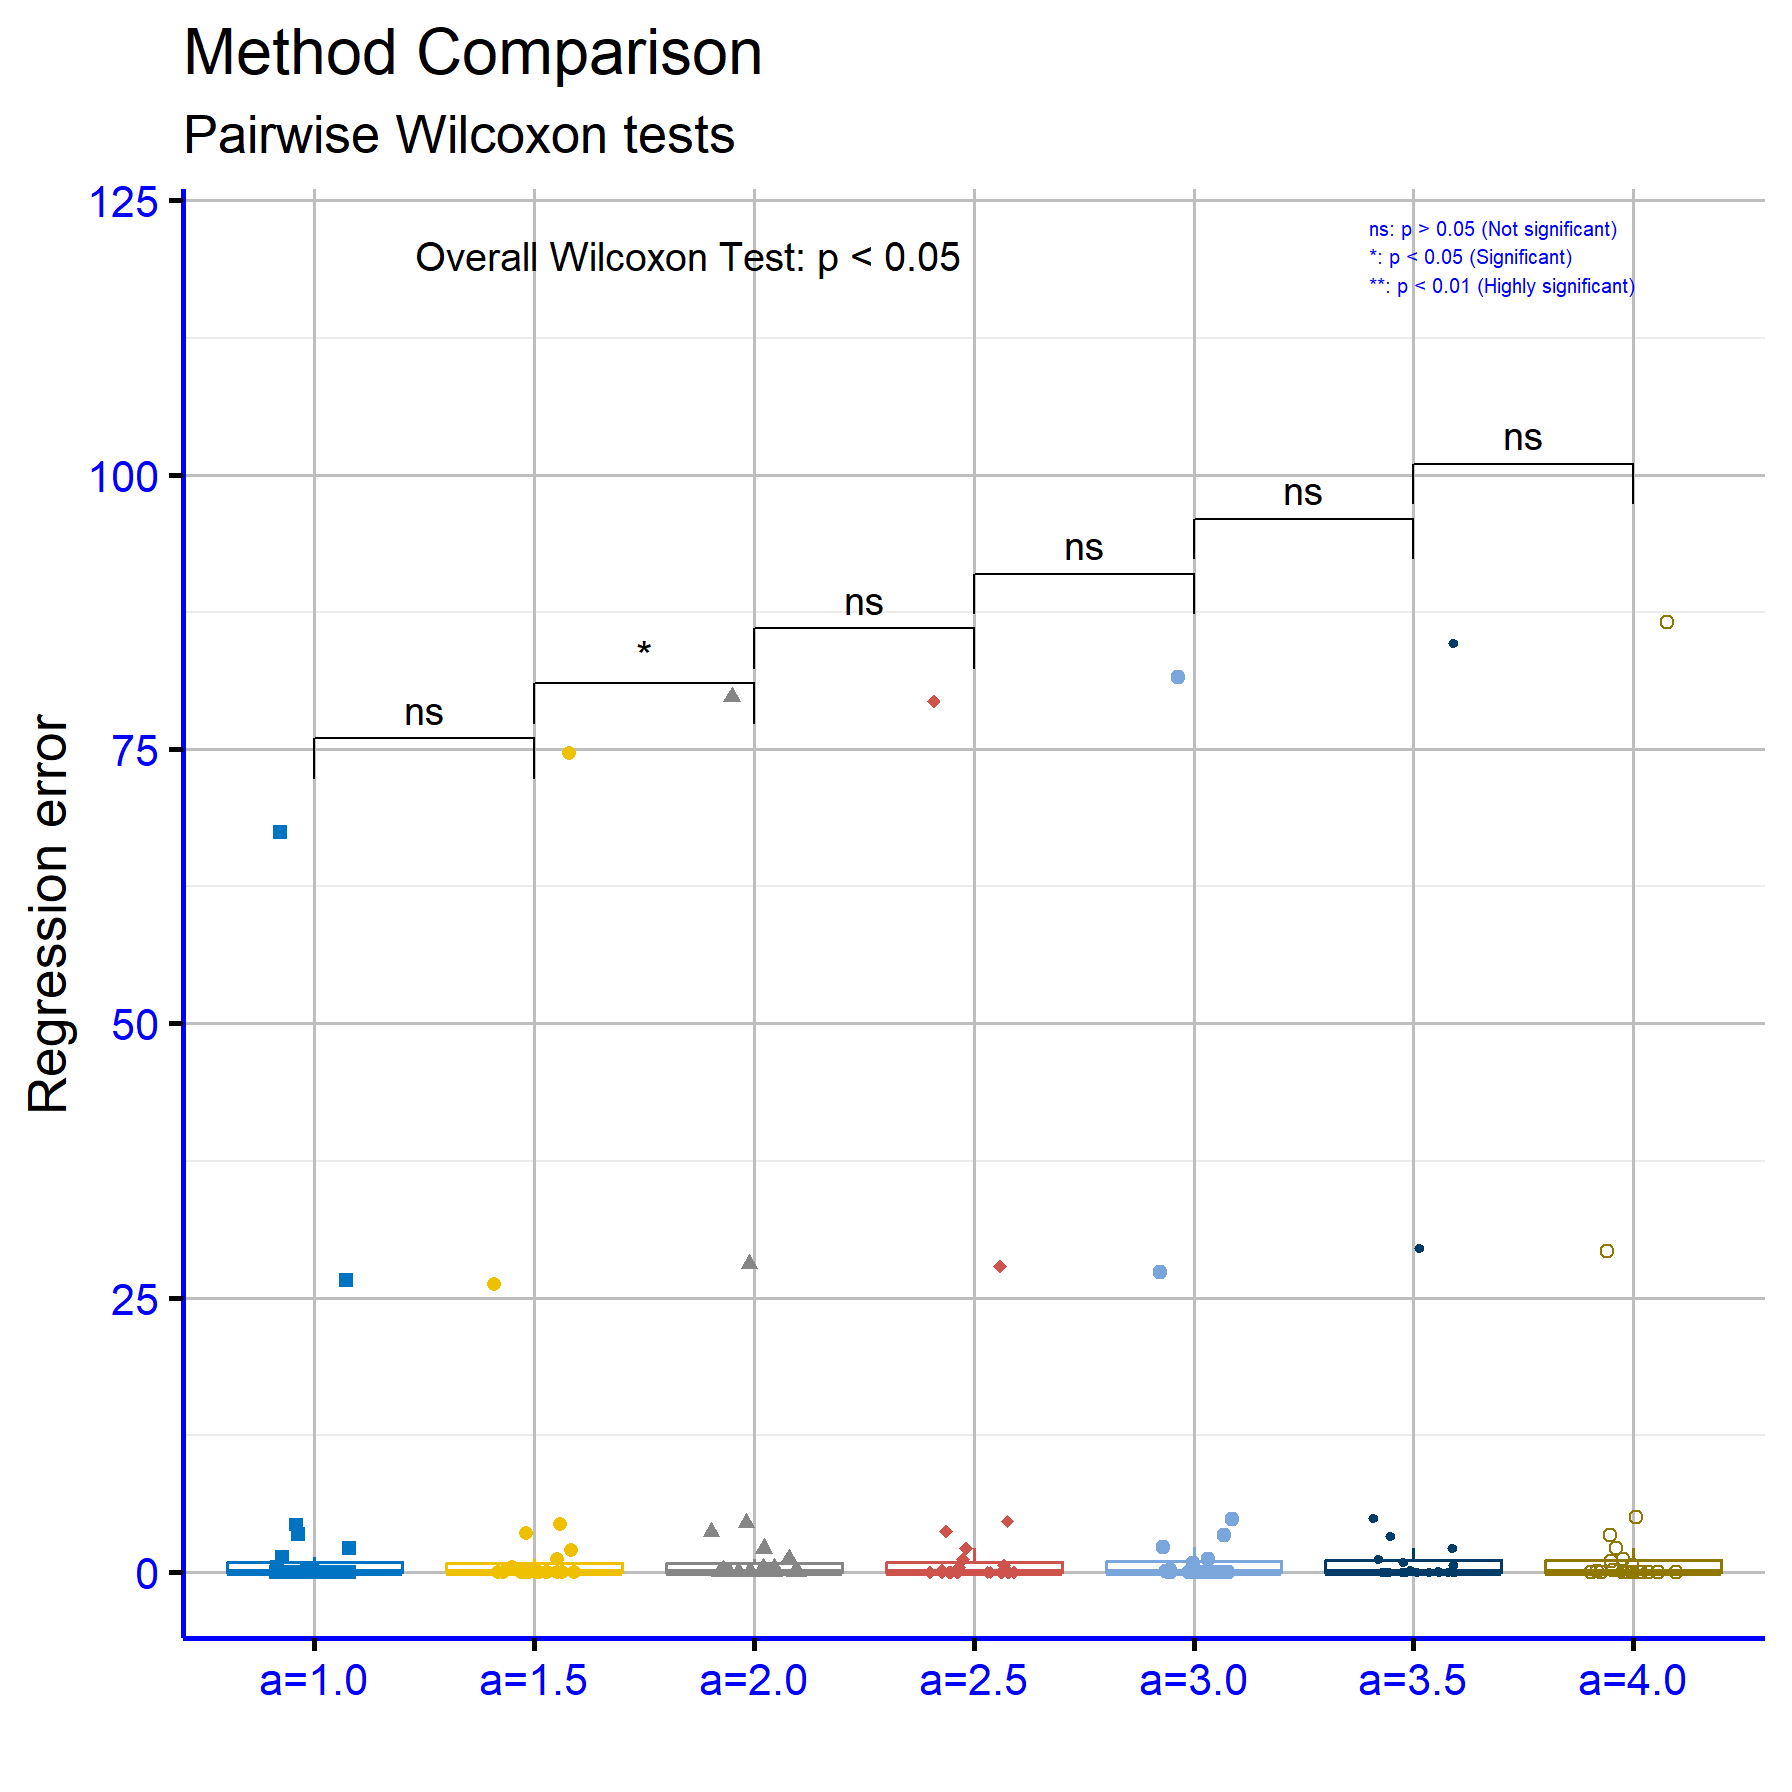
\includegraphics[scale=0.5]{img6}
\par\end{centering}
\caption{Statistical comparison for the experiments on the regression datasets,
using the proposed method and different values for the margin factor
$a$.\protect\label{fig:statRegressionA}}

\end{figure}

The table \ref{tab:ExperimentsClassificationA} presents the percentage
error values corresponding to various classification datasets for
different values of the parameter $a$ which determines the optimal
value boundaries in the proposed machine learning model. The last
row of the table includes the average error for each value of the
parameter $a$. The data analysis reveals that an increase in the
parameter $a$ generally leads to a rise in the average error rate.
Specifically, the average increases from 20.02\% for $\alpha=1.0$
to 21.38\% for $\alpha=3.5$, while for $\alpha=4.0$, it slightly
decreases to 21.00\%. This indicates that, despite the general upward
trend, there are cases where further increasing the parameter can
reduce the error. A detailed examination of the data by dataset shows
significant variations among different values of the parameter $a$.
For example, in the Circular dataset, the error gradually increases
from 3.69\% for $\alpha=1.0$ to 4.70\% for $\alpha=4.0$. Similarly,
in the Wine dataset, the error value increases from 8.55\% for $\alpha=1.0$
to 11.02\% for $\alpha=4.0$, indicating a clear negative impact of
increasing the parameter. However, in other datasets, the effect of
the parameter is neither as linear nor as pronounced. For instance,
in the Hayes Roth dataset, the error decreases from 39.69\% for $\alpha=2.0$
to 35.49\% for $\alpha=2.5$, before increasing again. Similarly,
in the Lymography dataset, the error significantly decreases for $\alpha=4.0$
(26.69\%) compared to the other parameter values. These data demonstrate
that the relationship between the parameter $a$ and the error is
not linear across all datasets and depends on the specific characteristics
of each dataset. Overall, the statistical analysis indicates that
while increasing the parameter $a$ is often associated with higher
errors, there are exceptions that may be linked to specific properties
of the data or the model.

The table \ref{tab:expRegressionA} presents the absolute error values
for various regression datasets in relation to different values of
the parameter $a$ which determines the optimal value boundaries in
the proposed machine learning model. The last row lists the average
errors for each value of the parameter $a$. The table analysis shows
that an increase in the parameter $a$ is accompanied by a general
increase in the average error. Specifically, the average error increases
from 4.64 for $\alpha=1.0$ to 5.64 for $\alpha=4.0$, suggesting
that higher parameter values may lead to worse model performance.
Examining the individual datasets reveals variability in the effect
of the parameter $a$. For example, in the BASEBALL dataset, the error
continuously increases from 67.45 for $\alpha=1.0$ to 86.54 for $\alpha=4.0$,
indicating a clear negative effect of increasing the parameter. Conversely,
in the STOCK dataset, an increase in the parameter is accompanied
by a decrease in error, from 3.47 for $\alpha=1.0$ to 3.35 for $\alpha=4.0$.
In other datasets, the effect is less straightforward. For example,
in the MORTGAGE dataset, the error increases from 0.31 for $\alpha=1.0$
to 0.68 for $\alpha=3.5$ but slightly decreases to 0.62 for $\alpha=4.0$.
Overall, the statistical analysis suggests that the effect of the
parameter $a$ depends on the characteristics of each dataset and
that, although increasing the parameter is often associated with higher
errors, there are cases where performance remains stable or improves
slightly.

In Figure \ref{fig:statClassA}, the results pertain to classification
datasets and various models. From the comparisons between different
values of the parameter $a$ it is observed that the comparison between
$a=1.0$ and $a=1.5$ does not exhibit a statistically significant
difference ($p=0.38$). In contrast, the comparison between $a=1.5$
and $a=2.0$ shows a significant difference ($p=0.018$), as does
the comparison between $a=2.0$ and $a=2.5$ ($p=0.045$). The remaining
comparisons, specifically between $a=2.5$ and $a=3.0$ ($p=0.25$),
$a=3.0$ and $a=3.5$ ($p=0.27$), and $a=3.5$ and $a=4.0$ ($p=0.39$),
do not demonstrate statistically significant differences.

In Figure \ref{fig:statRegressionA}, the data refer to regression
datasets and comparisons for various models. The results indicate
that the comparison between $a=1.0$ and $a=1.5$ is not statistically
significant ($p=0.55$), whereas the difference between $a=1.5$ and
$a=2.0$ is statistically significant ($p=0.014$). The comparison
between $a=2.0$ and $a=2.5$ does not show statistical significance
($p=0.17$), nor do the comparisons between $a=2.5$ and $a=3.0$
($p=0.2$), $a=3.0$ and $a=3.5$ ($p=0.16$), and $a=3.5$ and $a=4.0$
($p=0.31$). Overall, the $p$ values highlight significant differences
in specific cases, while in others, the differences remain statistically
insignificant.

\section{Conclusions \protect\label{sec:Conclusions}}

The study confirms the superiority of the proposed model compared
to existing methods in both classification and regression tasks. This
superiority is demonstrated by a statistically significant reduction
in error, although the model’s performance heavily depends on data
characteristics such as complexity, stratification, or the presence
of noise. This highlights the importance of adapting the model to
the specificities of each problem, as overly generalized approaches
may lead to suboptimal results. Additionally, the choice of methods
for calculating critical parameters, such as differential weights,
appears to have a relatively limited impact on overall performance.
Differences between approaches (e.g., FIXED, ADAPTIVE, RANDOM) are
minimal and often statistically insignificant, suggesting that optimization
efforts could focus on other factors. Tuning the parameter \textquotedbl a,\textquotedbl{}
however, emerges as a critical factor. Higher values of this parameter
often improve accuracy, particularly for large or complex datasets,
but they may also introduce instability in applications where data
sensitivity is high (e.g., financial forecasting). This dual behavior
underscores the need to balance flexibility and robustness during
the tuning process. Despite its analytical approach, the study does
not sufficiently explore the potential real-world applications of
the proposed model beyond benchmark datasets. Addressing this gap,
future research could expand the methodology to practical domains
such as biomedical data analysis, social networks, or dynamic systems,
including real-time monitoring and financial forecasting. Investigating
the model’s adaptability and scalability in these fields could enhance
its utility in real-world scenarios.

For future research, it would be beneficial to develop dynamic algorithms
that automatically adjust the parameter $a$ based on data dynamics.
For example, machine learning mechanisms that analyze data variability
or heterogeneity in real-time could optimize the value of $a$ without
human intervention, ensuring both stability and high performance.
Additionally, the development of hybrid methods that combine the adaptability
of ADAPTIVE approaches with the simplicity of FIXED approaches could
result in more resilient solutions capable of addressing a broader
range of problems. It is also important to investigate how specific
data characteristics---such as noisy measurements, class imbalances,
or lack of labeling---affect the model’s effectiveness. Such analysis
would support the development of adaptive strategies for data preprocessing
or augmentation. Furthermore, exploring the generalizability of results
to more complex environments, such as time-series data or dynamic
systems, remains an open research avenue. Finally, integrating explainable
artificial intelligence (XAI) techniques, such as feature contribution
analysis or visualization tools, could enhance the model’s transparency.
This would not only facilitate the interpretation of results by experts
but also aid in identifying optimal parameter-tuning practices, making
the model a more predictable and reliable tool for real-world applications.

\vspace{6pt}


\authorcontributions{V.C. and I.G.T. conducted the experiments, employing several datasets
and provided the comparative experiments. D.T. and V.C. performed
the statistical analysis and prepared the manuscript. All authors
have read and agreed to the published version of the manuscript.}

\funding{This research received no external funding.}

\institutionalreview{Not applicable.}

\informedconsent{Not applicable. }

\informedconsent{Not applicable. }

\acknowledgments{This research has been financed by the European Union : Next Generation
EU through the Program Greece 2.0 National Recovery and Resilience
Plan , under the call RESEARCH -- CREATE -- INNOVATE, project name
“iCREW: Intelligent small craft simulator for advanced crew training
using Virtual Reality techniques\textquotedbl{} (project code:TAEDK-06195).
\quad{}}

\conflictsofinterest{The authors declare no conflict of interest.}

\sampleavailability{Not applicable.}

\appendixtitles{no}

\appendixstart{}

\appendix

\begin{adjustwidth}{-\extralength}{0cm}{}


\reftitle{References}
\begin{thebibliography}{99}
\bibitem{nn1}Abiodun, O. I., Jantan, A., Omolara, A. E., Dada, K.
V., Mohamed, N. A., \& Arshad, H. (2018). State-of-the-art in artificial
neural network applications: A survey. Heliyon, 4(11).

\bibitem{nn2}Suryadevara, S., \& Yanamala, A. K. Y. (2021). A Comprehensive
Overview of Artificial Neural Networks: Evolution, Architectures,
and Applications. Revista de Inteligencia Artificial en Medicina,
12(1), 51-76.

\bibitem{nnphysics1}P. Baldi, K. Cranmer, T. Faucett et al, Parameterized
neural networks for high-energy physics, Eur. Phys. J. C \textbf{76},
2016.

\bibitem{nnphysics2}Baldi, P., Cranmer, K., Faucett, T., Sadowski,
P., \& Whiteson, D. (2016). Parameterized neural networks for high-energy
physics. The European Physical Journal C, 76(5), 1-7.

\bibitem{nnastro}Firth, A. E., Lahav, O., \& Somerville, R. S. (2003).
Estimating photometric redshifts with artificial neural networks.
Monthly Notices of the Royal Astronomical Society, 339(4), 1195-1202.

\bibitem{nnchem1}Shen, Y., \& Bax, A. (2013). Protein backbone and
sidechain torsion angles predicted from NMR chemical shifts using
artificial neural networks. Journal of biomolecular NMR, 56, 227-241.

\bibitem{nn_credit}Z. Huang, H. Chen, C.-Jung Hsu, W.-Hwa Chen, S.
Wu, Credit rating analysis with support vector machines and neural
networks: a market comparative study, Decision Support Systems \textbf{37},
pp. 543-558, 2004.

\bibitem{nnmed1}Igor I. Baskin, David Winkler and Igor V. Tetko,
A renaissance of neural networks in drug discovery, Expert Opinion
on Drug Discovery \textbf{11}, pp. 785-795, 2016.

\bibitem{nnmed2}Ronadl Bartzatt, Prediction of Novel Anti-Ebola Virus
Compounds Utilizing Artificial Neural Network (ANN), Chemistry Faculty
Publications \textbf{49}, pp. 16-34, 2018.

\bibitem{bpnn}D.E. Rumelhart, G.E. Hinton and R.J. Williams, Learning
representations by back-propagating errors, Nature \textbf{323}, pp.
533 - 536 , 1986.

\bibitem{bpnn2}T. Chen and S. Zhong, Privacy-Preserving Backpropagation
Neural Network Learning, IEEE Transactions on Neural Networks \textbf{20},
, pp. 1554-1564, 2009.

\bibitem{rpropnn}M. Riedmiller and H. Braun, A Direct Adaptive Method
for Faster Backpropagation Learning: The RPROP algorithm, Proc. of
the IEEE Intl. Conf. on Neural Networks, San Francisco, CA, pp. 586--591,
1993.

\bibitem{rpropnn3}T. Pajchrowski, K. Zawirski and K. Nowopolski,
Neural Speed Controller Trained Online by Means of Modified RPROP
Algorithm, IEEE Transactions on Industrial Informatics \textbf{11},
pp. 560-568, 2015.

\bibitem{rpropnn2}Rinda Parama Satya Hermanto, Suharjito, Diana,
Ariadi Nugroho, Waiting-Time Estimation in Bank Customer Queues using
RPROP Neural Networks, Procedia Computer Science \textbf{ 135}, pp.
35-42, 2018.

\bibitem{quasinn}B. Robitaille and B. Marcos and M. Veillette and
G. Payre, Modified quasi-Newton methods for training neural networks,
Computers \& Chemical Engineering \textbf{20}, pp. 1133-1140, 1996.

\bibitem{quasinn2}Q. Liu, J. Liu, R. Sang, J. Li, T. Zhang and Q.
Zhang, Fast Neural Network Training on FPGA Using Quasi-Newton Optimization
Method,IEEE Transactions on Very Large Scale Integration (VLSI) Systems
\textbf{26}, pp. 1575-1579, 2018.

\bibitem{nn_siman}C.L. Kuo, E.E. Kuruoglu, W.K.V. Chan, Neural Network
Structure Optimization by Simulated Annealing, Entropy \textbf{24},
348, 2022.

\bibitem{psonn}C. Zhang, H. Shao and Y. Li, Particle swarm optimisation
for evolving artificial neural network, IEEE International Conference
on Systems, Man, and Cybernetics, , pp. 2487-2490, 2000.

\bibitem{psonn2}Jianbo Yu, Shijin Wang, Lifeng Xi, Evolving artificial
neural networks using an improved PSO and DPSO \textbf{71}, pp. 1054-1060,
2008.

\bibitem{geneticnn}F. H. F. Leung, H. K. Lam, S. H. Ling and P. K.
S. Tam, Tuning of the structure and parameters of a neural network
using an improved genetic algorithm, IEEE Transactions on Neural Networks
\textbf{14}, pp. 79-88, 2003

\bibitem{geneticnn2}X. Yao, Evolving artificial neural networks,
Proceedings of the IEEE, 87(9), pp. 1423-1447, 1999.

\bibitem{weight_de1}Wang, L., Zeng, Y., \& Chen, T. (2015). Back
propagation neural network with adaptive differential evolution algorithm
for time series forecasting. Expert Systems with Applications, 42(2),
855-863.

\bibitem{weight_aco}K.M. Salama, A.M. Abdelbar, Learning neural network
structures with ant colony algorithms, Swarm Intell \textbf{9}, pp.
229--265, 2015.

\bibitem{gwo_nn}S. Mirjalili, How effective is the Grey Wolf optimizer
in training multi-layer perceptrons, Appl Intell \textbf{43}, pp.
150--161, 2015.

\bibitem{whale_nn}I. Aljarah, H. Faris, S. Mirjalili, Optimizing
connection weights in neural networks using the whale optimization
algorithm, Soft Comput \textbf{22}, pp. 1--15, 2018. 

\bibitem{nn_hybrid}J.-R. Zhang, J. Zhang, T.-M. Lok, M.R. Lyu, A
hybrid particle swarm optimization--back-propagation algorithm for
feedforward neural network training, Applied Mathematics and Computation
\textbf{185}, pp. 1026-1037, 2007.

\bibitem{nn_gpu1}K-Su Oh, K. Jung, GPU implementation of neural networks,
Pattern Recognition \textbf{37}, pp. 1311-1314, 2004.

\bibitem{nn_gpu2}M. Zhang, K. Hibi, J. Inoue, GPU-accelerated artificial
neural network potential for molecular dynamics simulation, Computer
Physics Communications \textbf{285}, 108655, 2023. 

\bibitem[(2017)]{lat}Krüger, T., Kusumaatmaja, H., Kuzmin, A., Shardt,
O., Silva, G., \& Viggen, E. M. (2017). The lattice Boltzmann method.
Springer International Publishing, 10(978-3), 4-15.

\bibitem[(2024)]{kang}Kang, Q., Li, K. Q., Fu, J. L., \& Liu, Y.
(2024). Hybrid LBM and machine learning algorithms for permeability
prediction of porous media: a comparative study. Computers and Geotechnics,
168, 106163.

\bibitem{weight_init1}I. Ivanova, M. Kubat, Initialization of neural
networks by means of decision trees, Knowledge-Based Systems \textbf{8},
pp. 333-344, 1995.

\bibitem{weight_init2}J.Y.F. Yam, T.W.S. Chow, A weight initialization
method for improving training speed in feedforward neural network,
Neurocomputing \textbf{30}, pp. 219-232, 2000.

\bibitem{weight_init3}K. Chumachenko, A. Iosifidis, M. Gabbouj, Feedforward
neural networks initialization based on discriminant learning, Neural
Networks \textbf{146}, pp. 220-229, 2022.

\bibitem{nn_init1}T.M. Varnava, A.J.Meade, An initialization method
for feedforward artificial neural networks using polynomial bases,
Advances in Adaptive Data Analysis \textbf{3}, pp. 385-400, 2011.

\bibitem{nn_init3}S.S. Sodhi, P. Chandra, Interval based Weight Initialization
Method for Sigmoidal Feedforward Artificial Neural Networks, AASRI
Procedia \textbf{6}, pp. 19-25, 2014.

\bibitem{nn_init_review}Narkhede, M. V., Bartakke, P. P., \& Sutaone,
M. S. (2022). A review on weight initialization strategies for neural
networks. Artificial intelligence review, 55(1), 291-322.

\bibitem{nn_arch1}J. Arifovic, R. Gençay, Using genetic algorithms
to select architecture of a feedforward artificial neural network,
Physica A: Statistical Mechanics and its Applications \textbf{289},
pp. 574-594, 2001.

\bibitem{nn_arch2}P.G. Benardos, G.C. Vosniakos, Optimizing feedforward
artificial neural network architecture, Engineering Applications of
Artificial Intelligence \textbf{20}, pp. 365-382, 2007.

\bibitem{nn_arch3}B.A. Garro, R.A. Vázquez, Designing Artificial
Neural Networks Using Particle Swarm Optimization Algorithms, Computational
Intelligence and Neuroscience, 369298, 2015. 

\bibitem{nn_arch4}B. Baker, O. Gupta, N. Naik, R. Raskar, Designing
neural network architectures using reinforcement learning. arXiv preprint
arXiv:1611.02167, 2016.

\bibitem{ge1}M. O’Neill, C. Ryan, Grammatical evolution, IEEE Trans.
Evol. Comput. \textbf{5,}pp. 349--358, 2001.

\bibitem{nnc}I.G. Tsoulos, D. Gavrilis, E. Glavas, Neural network
construction and training using grammatical evolution, Neurocomputing
\textbf{72}, pp. 269-277, 2008.

\bibitem{de_review}Pant, M., Zaheer, H., Garcia-Hernandez, L., \&
Abraham, A. (2020). Differential Evolution: A review of more than
two decades of research. Engineering Applications of Artificial Intelligence,
90, 103479.

\bibitem{de_symmetry1}Li, Y. H., Wang, J. Q., Wang, X. J., Zhao,
Y. L., Lu, X. H., \& Liu, D. L. (2017). Community detection based
on differential evolution using social spider optimization. Symmetry,
9(9), 183.

\bibitem{de_symmetry3}Yang, W., Siriwardane, E. M. D., Dong, R.,
Li, Y., \& Hu, J. (2021). Crystal structure prediction of materials
with high symmetry using differential evolution. Journal of Physics:
Condensed Matter, 33(45), 455902.

\bibitem{de_symmetry6}Lee, C. Y., \& Hung, C. H. (2021). Feature
ranking and differential evolution for feature selection in brushless
DC motor fault diagnosis. Symmetry, 13(7), 1291.

\bibitem{de_symmetry7}Saha, S., \& Das, R. (2018). Exploring differential
evolution and particle swarm optimization to develop some symmetry-based
automatic clustering techniques: application to gene clustering. Neural
Computing and Applications, 30, 735-757.

\bibitem{gen_app1}S.A. Grady, M.Y. Hussaini, M.M. Abdullah, Placement
of wind turbines using genetic algorithms, Renewable Energy \textbf{30},
pp. 259-270, 2005.

\bibitem{gen_app2}Prasad, T., Park, N., Multiobjective Genetic Algorithms
for Design of Water Distribution Networks, J. Water Resour. Plann.
Manage. \textbf{130}, pp. 73-82, 2004. 

\bibitem{gen_app3}Sung-Hwan Min, Jumin Lee, Ingoo Han, Hybrid genetic
algorithms and support vector machines for bankruptcy prediction,
Expert Systems with Applications \textbf{31}, pp. 652-660, 2006.

\bibitem{gen_app4}D. Whitley, T. Starkweather, C. Bogart, Genetic
algorithms and neural networks: Optimizing connections and connectivity,
Parallel Computing \textbf{14}, pp. 347-361, 1990.

\bibitem{kaelo}P. Kaelo, M.M. Ali, Integrated crossover rules in
real coded genetic algorithms, European Journal of Operational Research
\textbf{176}, pp. 60-76, 2007.

\bibitem{UCL}M. Kelly, R. Longjohn, K. Nottingham, The UCI Machine
Learning Repository. 2023. Available online: https://archive.ics.uci.edu
(accessed on 20 September 2023).

\bibitem{Keel}J. Alcalá-Fdez, A. Fernandez, J. Luengo, J. Derrac,
S. García, L. Sánchez, F. Herrera. KEEL Data-Mining Software Tool:
Data Set Repository, Integration of Algorithms and Experimental Analysis
Framework. Journal of Multiple-Valued Logic and Soft Computing 17,
pp. 255-287, 2011.

\bibitem[Tzimourta(2018)]{alcohol}Tzimourta, K.D.; Tsoulos, I.; Bilero,
I.T.; Tzallas, A.T.; Tsipouras, M.G.; Giannakeas, N. Direct Assessment
of Alcohol Consumption in Mental State Using Brain Computer Interfaces
and Grammatical Evolution. Inventions 2018, 3, 51.

\bibitem{appendicitis}Weiss, Sholom M. and Kulikowski, Casimir A.,
Computer Systems That Learn: Classification and Prediction Methods
from Statistics, Neural Nets, Machine Learning, and Expert Systems,
Morgan Kaufmann Publishers Inc, 1991.

\bibitem[Quinlan(2018)]{australian}J.R. Quinlan, Simplifying Decision
Trees. International Journal of Man-Machine Studies \textbf{27}, pp.
221-234, 1987. 

\bibitem{balance}T. Shultz, D. Mareschal, W. Schmidt, Modeling Cognitive
Development on Balance Scale Phenomena, Machine Learning \textbf{16},
pp. 59-88, 1994.

\bibitem[(2004)]{cleveland1}Z.H. Zhou,Y. Jiang, NeC4.5: neural ensemble
based C4.5,\textquotedbl{} in IEEE Transactions on Knowledge and Data
Engineering \textbf{16}, pp. 770-773, 2004.

\bibitem{cleveland2}R. Setiono , W.K. Leow, FERNN: An Algorithm for
Fast Extraction of Rules from Neural Networks, Applied Intelligence
\textbf{12}, pp. 15-25, 2000.

\bibitem[(1998)]{dermatology}G. Demiroz, H.A. Govenir, N. Ilter,
Learning Differential Diagnosis of Eryhemato-Squamous Diseases using
Voting Feature Intervals, Artificial Intelligence in Medicine. \textbf{13},
pp. 147--165, 1998.

\bibitem[(1996)]{ecoli}P. Horton, K.Nakai, A Probabilistic Classification
System for Predicting the Cellular Localization Sites of Proteins,
In: Proceedings of International Conference on Intelligent Systems
for Molecular Biology \textbf{4}, pp. 109-15, 1996.

\bibitem[(1977)]{hayes-roth}B. Hayes-Roth, B., F. Hayes-Roth. Concept
learning and the recognition and classification of exemplars. Journal
of Verbal Learning and Verbal Behavior \textbf{16}, pp. 321-338, 1977.

\bibitem[(1997)]{heart}I. Kononenko, E. Šimec, M. Robnik-Šikonja,
Overcoming the Myopia of Inductive Learning Algorithms with RELIEFF,
Applied Intelligence \textbf{7}, pp. 39--55, 1997.

\bibitem[(2002)]{housevotes}R.M. French, N. Chater, Using noise to
compute error surfaces in connectionist networks: a novel means of
reducing catastrophic forgetting, Neural Comput. \textbf{14}, pp.
1755-1769, 2002.

\bibitem[(2004)]{ion1}J.G. Dy , C.E. Brodley, Feature Selection for
Unsupervised Learning, The Journal of Machine Learning Research \textbf{5},
pp 845--889, 2004.

\bibitem{ion2}S. J. Perantonis, V. Virvilis, Input Feature Extraction
for Multilayered Perceptrons Using Supervised Principal Component
Analysis, Neural Processing Letters \textbf{10}, pp 243--252, 1999.

\bibitem[(2002)]{liver1} J. Garcke, M. Griebel, Classification with
sparse grids using simplicial basis functions, Intell. Data Anal.
\textbf{6}, pp. 483-502, 2002.

\bibitem{liver2}J. Mcdermott, R.S. Forsyth, Diagnosing a disorder
in a classification benchmark, Pattern Recognition Letters \textbf{73},
pp. 41-43, 2016.

\bibitem[(2002)]{lymography}G. Cestnik, I. Konenenko, I. Bratko,
Assistant-86: A Knowledge-Elicitation Tool for Sophisticated Users.
In: Bratko, I. and Lavrac, N., Eds., Progress in Machine Learning,
Sigma Press, Wilmslow, pp. 31-45, 1987. 

\bibitem[(2007)]{mammographic}M. Elter, R. Schulz-Wendtland, T. Wittenberg,
The prediction of breast cancer biopsy outcomes using two CAD approaches
that both emphasize an intelligible decision process, Med Phys. \textbf{34},
pp. 4164-72, 2007.

\bibitem[(2007)]{parkinsons1}M.A. Little, P.E. McSharry, S.J Roberts
et al, Exploiting Nonlinear Recurrence and Fractal Scaling Properties
for Voice Disorder Detection. BioMed Eng OnLine \textbf{6}, 23, 2007.

\bibitem{parkinsons2}M.A. Little, P.E. McSharry, E.J. Hunter, J.
Spielman, L.O. Ramig, Suitability of dysphonia measurements for telemonitoring
of Parkinson's disease. IEEE Trans Biomed Eng. \textbf{56}, pp. 1015-1022,
2009.

\bibitem[(2007)]{pima}J.W. Smith, J.E. Everhart, W.C. Dickson, W.C.
Knowler, R.S. Johannes, Using the ADAP learning algorithm to forecast
the onset of diabetes mellitus, In: Proceedings of the Symposium on
Computer Applications and Medical Care IEEE Computer Society Press,
pp.261-265, 1988.

\bibitem[(2007)]{popfailures}D.D. Lucas, R. Klein, J. Tannahill,
D. Ivanova, S. Brandon, D. Domyancic, Y. Zhang, Failure analysis of
parameter-induced simulation crashes in climate models, Geoscientific
Model Development \textbf{6}, pp. 1157-1171, 2013.

\bibitem[(2007)]{regions2}N. Giannakeas, M.G. Tsipouras, A.T. Tzallas,
K. Kyriakidi, Z.E. Tsianou, P. Manousou, A. Hall, E.C. Karvounis,
V. Tsianos, E. Tsianos, A clustering based method for collagen proportional
area extraction in liver biopsy images (2015) Proceedings of the Annual
International Conference of the IEEE Engineering in Medicine and Biology
Society, EMBS, 2015-November, art. no. 7319047, pp. 3097-3100. 

\bibitem[(2007)]{saheart}T. Hastie, R. Tibshirani, Non-parametric
logistic and proportional odds regression, JRSS-C (Applied Statistics)
\textbf{36}, pp. 260--276, 1987.

\bibitem{segment}M. Dash, H. Liu, P. Scheuermann, K. L. Tan, Fast
hierarchical clustering and its validation, Data \& Knowledge Engineering
\textbf{44}, pp 109--138, 2003.

\bibitem{sonar}Gorman, R.P.; Sejnowski, T.J. Analysis of Hidden Units
in a Layered Network Trained to Classify Sonar Targets. Neural Netw.
1988, 1, 75--89.

\bibitem{student}P. Cortez, A. M. Gonçalves Silva, Using data mining
to predict secondary school student performance, In Proceedings of
5th FUture BUsiness TEChnology Conference (FUBUTEC 2008) (pp. 5--12).
EUROSIS-ETI, 2008.

\bibitem{wdbc}W.H. Wolberg, O.L. Mangasarian, Multisurface method
of pattern separation for medical diagnosis applied to breast cytology,
Proc Natl Acad Sci U S A. \textbf{87}, pp. 9193--9196, 1990.

\bibitem{wine1}M. Raymer, T.E. Doom, L.A. Kuhn, W.F. Punch, Knowledge
discovery in medical and biological datasets using a hybrid Bayes
classifier/evolutionary algorithm. IEEE transactions on systems, man,
and cybernetics. Part B, Cybernetics : a publication of the IEEE Systems,
Man, and Cybernetics Society, \textbf{33} , pp. 802-813, 2003.

\bibitem{wine2}P. Zhong, M. Fukushima, Regularized nonsmooth Newton
method for multi-class support vector machines, Optimization Methods
and Software \textbf{22}, pp. 225-236, 2007.

\bibitem[(2007)]{eeg1}R. G. Andrzejak, K. Lehnertz, F.Mormann, C.
Rieke, P. David, and C. E. Elger, “Indications of nonlinear deterministic
and finite-dimensional structures in time series of brain electrical
activity: dependence on recording region and brain state,” Physical
Review E, vol. 64, no. 6, Article ID 061907, 8 pages, 2001. 

\bibitem{eeg2}A. T. Tzallas, M. G. Tsipouras, and D. I. Fotiadis,
“Automatic Seizure Detection Based on Time-Frequency Analysis and
Artificial Neural Networks,” Computational Intelligence and Neuroscience,
vol. 2007, Article ID 80510, 13 pages, 2007. doi:10.1155/2007/80510.

\bibitem[(2007)]{zoo}M. Koivisto, K. Sood, Exact Bayesian Structure
Discovery in Bayesian Networks, The Journal of Machine Learning Research\textbf{
5}, pp. 549--573, 2004.

\bibitem[(2007)]{abalone}Nash, W.J.; Sellers, T.L.; Talbot, S.R.;
Cawthor, A.J.; Ford, W.B. The Population Biology of Abalone (\_Haliotis\_
species) in Tasmania. I. Blacklip Abalone (\_H. rubra\_) from the
North Coast and Islands of Bass Strait, Sea Fisheries Division; Technical
Report No. 48; Department of Primary Industry and Fisheries, Tasmania:
Hobart, Australia, 1994; ISSN 1034-3288

\bibitem[(2007)]{airfoil}Brooks, T.F.; Pope, D.S.; Marcolini, A.M.
Airfoil Self-Noise and Prediction. Technical Report, NASA RP-1218.
July 1989. Available online: https://ntrs.nasa.gov/citations/19890016302
(accessed on 5 March 2025).

\bibitem{BK}J.S. Simonoff, Smooting Methods in Statistics, Springer
- Verlag, 1996.

\bibitem{concrete}I.Cheng Yeh, Modeling of strength of high performance
concrete using artificial neural networks, Cement and Concrete Research.
\textbf{28}, pp. 1797-1808, 1998. 

\bibitem{housing}D. Harrison and D.L. Rubinfeld, Hedonic prices and
the demand for clean ai, J. Environ. Economics \& Management \textbf{5},
pp. 81-102, 1978.

\bibitem{friedman}Friedman, J. (1991): Multivariate Adaptative Regression
Splines. Annals of Statistics, 19:1, 1-{}-141. 

\bibitem{pydataset}R.D. King, S. Muggleton, R. Lewis, M.J.E. Sternberg,
Proc. Nat. Acad. Sci. USA \textbf{89}, pp. 11322--11326, 1992. 

\bibitem{nn_adam}D. P. Kingma, J. L. Ba, ADAM: a method for stochastic
optimization, in: Proceedings of the 3rd International Conference
on Learning Representations (ICLR 2015), pp. 1--15, 2015.

\bibitem{powell}M.J.D Powell, A Tolerant Algorithm for Linearly Constrained
Optimization Calculations, Mathematical Programming \textbf{45}, pp.
547-566, 1989. 

\bibitem{neat}K. O. Stanley, R. Miikkulainen, Evolving Neural Networks
through Augmenting Topologies, Evolutionary Computation \textbf{10},
pp. 99-127, 2002.

\bibitem[(1994)]{de_original}Storn, R., \& Price, K. (1997). Differential
evolution--a simple and efficient heuristic for global optimization
over continuous spaces. Journal of global optimization, 11, 341-359.

\bibitem{de_adaptive}Wu, K., Liu, Z., Ma, N., \& Wang, D. (2022).
A Dynamic Adaptive Weighted Differential Evolutionary Algorithm. Computational
Intelligence and Neuroscience, 2022(1), 1318044.

\bibitem{de_char}Charilogis V, Tsoulos IG, Tzallas A, Karvounis E.
Modifications for the Differential Evolution Algorithm. Symmetry.
2022; 14(3):447.

\end{thebibliography}
%%%%%%%%%%%%%%%%%%%%%%%%%%%%%%%%%%%%%%%%%%
%% for journal Sci
%\reviewreports{\\
%Reviewer 1 comments and authors' response\\
%Reviewer 2 comments and authors' response\\
%Reviewer 3 comments and authors' response
%}
%%%%%%%%%%%%%%%%%%%%%%%%%%%%%%%%%%%%%%%%%%

\PublishersNote{}

\end{adjustwidth}{}
\end{document}
